\documentclass[letterpaper,11pt]{article}

\usepackage{geometry}
\usepackage{pslatex}
\usepackage{fancyhdr}
\usepackage{graphicx}
\usepackage{color}
\usepackage{tikz}
\usepackage{setspace}
\usepackage{amssymb}

\geometry{ margin = 1.0in }

\pagestyle{fancy}
\lhead{{\bf Lecture 35}}
\chead{{\bf CMPSC 465 Fall 2020}}
\rhead{{\bf Mingfu Shao}}

\setlength\parindent{0em}
\setlength\parskip{8pt}
%\setlength{\fboxsep}{6pt}

\usepackage{amsthm}
\newtheoremstyle{mytheorem}
  {\parskip} % Space above
  {0em} % Space below
  {} % Body font
  {} % Indent amount
  {\bfseries} % Theorem head font
  {.} % Punctuation after theorem head
  {.5em} % Space after theorem head
  {} % Theorem head spec (can be left empty, meaning `normal')

\theoremstyle{mytheorem}
\newtheorem{definition}{Definition}
\newtheorem{property}{Property}
\newtheorem{claim}{Claim}
\newtheorem{fact}{Fact}
\newtheorem{corollary}{Corollary}

% for algorithms
\newcommand{\aaa}[1]{\hspace{0.65cm}\parbox[t]{15.3cm}{#1}}
\newcommand{\aab}[1]{\hspace{1.15cm}\parbox[t]{15.0cm}{#1}}
\newcommand{\aac}[1]{\hspace{1.65cm}\parbox[t]{15.0cm}{#1}}
\newcommand{\aad}[1]{\hspace{2.15cm}\parbox[t]{15.0cm}{#1}}
\newcommand{\aae}[1]{\hspace{2.65cm}\parbox[t]{15.0cm}{#1}}
\newcommand{\aaf}[1]{\hspace{3.15cm}\parbox[t]{15.0cm}{#1}}
\newcommand{\aaA}[2]{\hspace{0.5cm} {\tikz[overlay] \draw (0.1, -0.1) -- (0.1, #1 * -1.5em + 0.6em);} \parbox[t]{15.0cm}{#2}}
\newcommand{\aaB}[2]{\hspace{1.0cm} {\tikz[overlay] \draw (0.1, -0.1) -- (0.1, #1 * -1.5em + 0.6em);} \parbox[t]{15.0cm}{#2}}
\newcommand{\aaC}[2]{\hspace{1.5cm} {\tikz[overlay] \draw (0.1, -0.1) -- (0.1, #1 * -1.5em + 0.6em);} \parbox[t]{15.0cm}{#2}}
\newcommand{\aaD}[2]{\hspace{2.0cm} {\tikz[overlay] \draw (0.1, -0.1) -- (0.1, #1 * -1.5em + 0.6em);} \parbox[t]{15.0cm}{#2}}
\newcommand{\aaE}[2]{\hspace{2.5cm} {\tikz[overlay] \draw (0.1, -0.1) -- (0.1, #1 * -1.5em + 0.6em);} \parbox[t]{15.0cm}{#2}}
\newcommand{\xxx}{\par\vspace{0.1cm}}

\begin{document}

\section*{Vertex Cover Problem}

\subsection*{Addressing Hard Problems}

The vertex cover problem~(formally defined below), is one of the
so-called~\emph{NP-hard} problems.  The 3SAT problem and the Knapsack problem
we introduced before are also in this category.  Informally, a problem is
{NP-hard} means that \emph{there does not exist any polynomial-time (optimal)
algorithm for it}. To address a NP-hard problem, we therefore have to either
drop polynomial-time constraint or drop optimality.

\vspace*{-\topsep}
\begin{enumerate}
\item Design optimal algorithms but don't run in polynomial-time.
For example, for the knapsack problem, we designed a DP algorithm~(which
is optimal), but runs in $O(nW)$ time, which is exponential.
\item Design polynomial-time algorithms but are not optimal.
We usually require that, the solution obtained is \emph{guaranteed
to be close to the optimal solution}; we call them \emph{approximation algorithms}.
\end{enumerate}

Here is a formal description of \emph{approximation algorithm}.
Let $P$ be an optimization problem and assume the objective
is to \emph{minimize} a function.
Let $\mathcal{A}$ be an algorithm for problem $P$. We say $\mathcal{A}$
is an approximation algorithm of $P$ with \emph{approximation ratio} of $c$, if for \emph{every} instance
$I$ of $P$, we have $\mathcal{A}(I) / opt(I) \le c$,
where $\mathcal{A}(I)$ represents the solution produced by algorithm $\mathcal{A}$ given instance $I$,
and $opt(I)$ represents the optimal solution of instance $I$.

Below, we will design greedy algorithms for the vertex cover problem, and
prove that they are actually approximation algorithms~(with different approximation ratios).
%by showing that $\mathcal{A}(I) / opt(I) \le c$ for every instance.

\subsection*{The Problem}

Let $G = (V, E)$ be an undirected graph. We say a subset $V_1\subset V$
\emph{covers} all edges of $E$, if for \emph{every} edge $(u,v)\in E$,
either we have $u\in V_1$, or $v\in V_1$, or both.
Given undirected graph $G = (V, E)$,
the \emph{vertex cover problem} seeks $V_1\subset V$ that covers $E$
and that $|V_1|$ is minimized. See Figure~\ref{fig:cover}.

\begin{figure}[h]
\centering{

\tikzset{every picture/.style={line width=0.75pt}} %set default line width to 0.75pt        

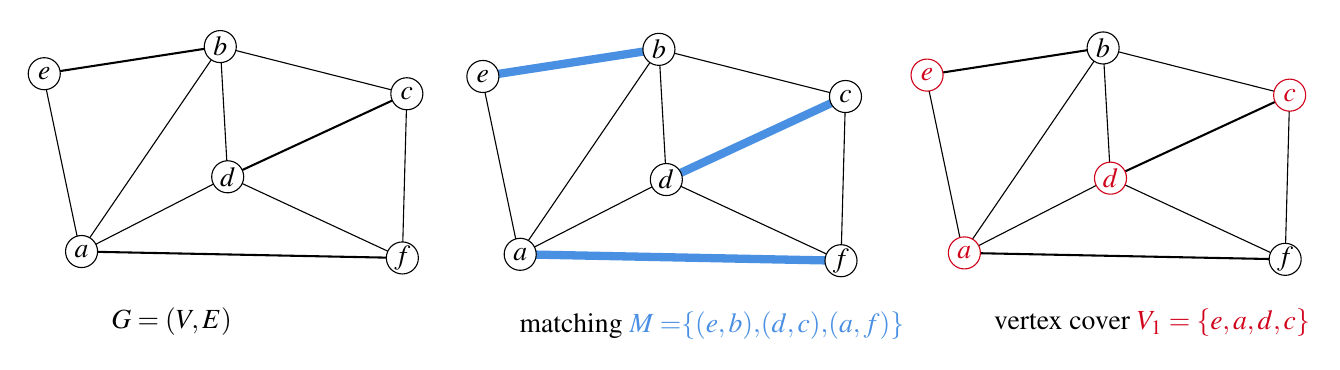
\begin{tikzpicture}[x=0.5pt,y=0.5pt,yscale=-1,xscale=1]
%uncomment if require: \path (0,237); %set diagram left start at 0, and has height of 237

%Straight Lines [id:da7485926733039977] 
\draw    (144.6,14.97) -- (43.43,163.09) ;
%Straight Lines [id:da4575120980127291] 
\draw [color={rgb, 255:red, 0; green, 0; blue, 0 }  ,draw opacity=1 ][line width=0.75]    (16.46,34.58) -- (143.69,14.97) ;
%Straight Lines [id:da9165715401778428] 
\draw    (16.46,34.58) -- (43.43,163.09) ;
%Straight Lines [id:da994182434786223] 
\draw [color={rgb, 255:red, 0; green, 0; blue, 0 }  ,draw opacity=1 ][line width=0.75]    (44.34,163.09) -- (276.17,167.73) ;
%Straight Lines [id:da9750224919648968] 
\draw    (149.95,109.07) -- (276.17,167.73) ;
%Straight Lines [id:da24348552449211425] 
\draw    (144.6,14.97) -- (149.95,109.07) ;
%Straight Lines [id:da16705340438790406] 
\draw    (144.6,14.97) -- (279.42,49.07) ;
%Straight Lines [id:da08663700279220432] 
\draw    (279.42,49.07) -- (276.17,167.73) ;
%Straight Lines [id:da16511775802360662] 
\draw [color={rgb, 255:red, 0; green, 0; blue, 0 }  ,draw opacity=1 ][line width=0.75]    (279.42,49.07) -- (149.95,109.07) ;
%Straight Lines [id:da4151454155794566] 
\draw    (149.95,109.07) -- (44.34,163.09) ;
%Shape: Ellipse [id:dp9133580928774087] 
\draw  [fill={rgb, 255:red, 255; green, 255; blue, 255 }  ,fill opacity=1 ] (5.79,34.58) .. controls (5.79,28.18) and (10.97,23) .. (17.37,23) .. controls (23.76,23) and (28.95,28.18) .. (28.95,34.58) .. controls (28.95,40.97) and (23.76,46.16) .. (17.37,46.16) .. controls (10.97,46.16) and (5.79,40.97) .. (5.79,34.58) -- cycle ;
%Shape: Ellipse [id:dp4005957609675306] 
\draw  [fill={rgb, 255:red, 255; green, 255; blue, 255 }  ,fill opacity=1 ] (133.02,14.97) .. controls (133.02,8.57) and (138.2,3.39) .. (144.6,3.39) .. controls (151,3.39) and (156.18,8.57) .. (156.18,14.97) .. controls (156.18,21.36) and (151,26.55) .. (144.6,26.55) .. controls (138.2,26.55) and (133.02,21.36) .. (133.02,14.97) -- cycle ;
%Shape: Ellipse [id:dp49214617921702164] 
\draw  [fill={rgb, 255:red, 255; green, 255; blue, 255 }  ,fill opacity=1 ] (267.84,49.07) .. controls (267.84,42.67) and (273.02,37.49) .. (279.42,37.49) .. controls (285.82,37.49) and (291,42.67) .. (291,49.07) .. controls (291,55.46) and (285.82,60.65) .. (279.42,60.65) .. controls (273.02,60.65) and (267.84,55.46) .. (267.84,49.07) -- cycle ;
%Shape: Ellipse [id:dp8440754424343925] 
\draw  [fill={rgb, 255:red, 255; green, 255; blue, 255 }  ,fill opacity=1 ] (138.37,109.07) .. controls (138.37,102.68) and (143.55,97.49) .. (149.95,97.49) .. controls (156.34,97.49) and (161.53,102.68) .. (161.53,109.07) .. controls (161.53,115.47) and (156.34,120.65) .. (149.95,120.65) .. controls (143.55,120.65) and (138.37,115.47) .. (138.37,109.07) -- cycle ;
%Shape: Ellipse [id:dp20660183368429152] 
\draw  [fill={rgb, 255:red, 255; green, 255; blue, 255 }  ,fill opacity=1 ] (32.76,163.09) .. controls (32.76,156.7) and (37.94,151.51) .. (44.34,151.51) .. controls (50.73,151.51) and (55.92,156.7) .. (55.92,163.09) .. controls (55.92,169.49) and (50.73,174.67) .. (44.34,174.67) .. controls (37.94,174.67) and (32.76,169.49) .. (32.76,163.09) -- cycle ;
%Shape: Ellipse [id:dp4098192910838151] 
\draw  [fill={rgb, 255:red, 255; green, 255; blue, 255 }  ,fill opacity=1 ] (264.59,167.73) .. controls (264.59,161.33) and (269.77,156.15) .. (276.17,156.15) .. controls (282.56,156.15) and (287.75,161.33) .. (287.75,167.73) .. controls (287.75,174.13) and (282.56,179.31) .. (276.17,179.31) .. controls (269.77,179.31) and (264.59,174.13) .. (264.59,167.73) -- cycle ;
%Straight Lines [id:da6233481480623783] 
\draw    (461.6,16.97) -- (360.43,165.09) ;
%Straight Lines [id:da9901942575404544] 
\draw [color={rgb, 255:red, 74; green, 144; blue, 226 }  ,draw opacity=1 ][line width=3]    (333.46,36.58) -- (460.69,16.97) ;
%Straight Lines [id:da3790939323014558] 
\draw    (333.46,36.58) -- (360.43,165.09) ;
%Straight Lines [id:da42115713644274366] 
\draw [color={rgb, 255:red, 74; green, 144; blue, 226 }  ,draw opacity=1 ][line width=3]    (361.34,165.09) -- (593.17,169.73) ;
%Straight Lines [id:da8702690824311631] 
\draw    (466.95,111.07) -- (593.17,169.73) ;
%Straight Lines [id:da34939805445985417] 
\draw    (461.6,16.97) -- (466.95,111.07) ;
%Straight Lines [id:da04544520748950576] 
\draw    (461.6,16.97) -- (596.42,51.07) ;
%Straight Lines [id:da5361594760285122] 
\draw    (596.42,51.07) -- (593.17,169.73) ;
%Straight Lines [id:da10465085418843478] 
\draw [color={rgb, 255:red, 74; green, 144; blue, 226 }  ,draw opacity=1 ][line width=3]    (596.42,51.07) -- (466.95,111.07) ;
%Straight Lines [id:da555393377892622] 
\draw    (466.95,111.07) -- (361.34,165.09) ;
%Shape: Ellipse [id:dp39324544068995604] 
\draw  [fill={rgb, 255:red, 255; green, 255; blue, 255 }  ,fill opacity=1 ] (322.79,36.58) .. controls (322.79,30.18) and (327.97,25) .. (334.37,25) .. controls (340.76,25) and (345.95,30.18) .. (345.95,36.58) .. controls (345.95,42.97) and (340.76,48.16) .. (334.37,48.16) .. controls (327.97,48.16) and (322.79,42.97) .. (322.79,36.58) -- cycle ;
%Shape: Ellipse [id:dp8663152391911655] 
\draw  [fill={rgb, 255:red, 255; green, 255; blue, 255 }  ,fill opacity=1 ] (450.02,16.97) .. controls (450.02,10.57) and (455.2,5.39) .. (461.6,5.39) .. controls (468,5.39) and (473.18,10.57) .. (473.18,16.97) .. controls (473.18,23.36) and (468,28.55) .. (461.6,28.55) .. controls (455.2,28.55) and (450.02,23.36) .. (450.02,16.97) -- cycle ;
%Shape: Ellipse [id:dp9564869279164044] 
\draw  [fill={rgb, 255:red, 255; green, 255; blue, 255 }  ,fill opacity=1 ] (584.84,51.07) .. controls (584.84,44.67) and (590.02,39.49) .. (596.42,39.49) .. controls (602.82,39.49) and (608,44.67) .. (608,51.07) .. controls (608,57.46) and (602.82,62.65) .. (596.42,62.65) .. controls (590.02,62.65) and (584.84,57.46) .. (584.84,51.07) -- cycle ;
%Shape: Ellipse [id:dp14244956479013948] 
\draw  [fill={rgb, 255:red, 255; green, 255; blue, 255 }  ,fill opacity=1 ] (455.37,111.07) .. controls (455.37,104.68) and (460.55,99.49) .. (466.95,99.49) .. controls (473.34,99.49) and (478.53,104.68) .. (478.53,111.07) .. controls (478.53,117.47) and (473.34,122.65) .. (466.95,122.65) .. controls (460.55,122.65) and (455.37,117.47) .. (455.37,111.07) -- cycle ;
%Shape: Ellipse [id:dp3916752397044988] 
\draw  [fill={rgb, 255:red, 255; green, 255; blue, 255 }  ,fill opacity=1 ] (349.76,165.09) .. controls (349.76,158.7) and (354.94,153.51) .. (361.34,153.51) .. controls (367.73,153.51) and (372.92,158.7) .. (372.92,165.09) .. controls (372.92,171.49) and (367.73,176.67) .. (361.34,176.67) .. controls (354.94,176.67) and (349.76,171.49) .. (349.76,165.09) -- cycle ;
%Shape: Ellipse [id:dp6775141746120102] 
\draw  [fill={rgb, 255:red, 255; green, 255; blue, 255 }  ,fill opacity=1 ] (581.59,169.73) .. controls (581.59,163.33) and (586.77,158.15) .. (593.17,158.15) .. controls (599.56,158.15) and (604.75,163.33) .. (604.75,169.73) .. controls (604.75,176.13) and (599.56,181.31) .. (593.17,181.31) .. controls (586.77,181.31) and (581.59,176.13) .. (581.59,169.73) -- cycle ;
%Straight Lines [id:da991028078692109] 
\draw    (782.6,15.97) -- (681.43,164.09) ;
%Straight Lines [id:da8020042074548936] 
\draw [color={rgb, 255:red, 0; green, 0; blue, 0 }  ,draw opacity=1 ][line width=0.75]    (654.46,35.58) -- (781.69,15.97) ;
%Straight Lines [id:da5410354625843318] 
\draw    (654.46,35.58) -- (681.43,164.09) ;
%Straight Lines [id:da1284005435452643] 
\draw [color={rgb, 255:red, 0; green, 0; blue, 0 }  ,draw opacity=1 ][line width=0.75]    (682.34,164.09) -- (914.17,168.73) ;
%Straight Lines [id:da4841445577516499] 
\draw    (787.95,110.07) -- (914.17,168.73) ;
%Straight Lines [id:da3189236797568633] 
\draw    (782.6,15.97) -- (787.95,110.07) ;
%Straight Lines [id:da24633327282247075] 
\draw    (782.6,15.97) -- (917.42,50.07) ;
%Straight Lines [id:da666695835406161] 
\draw    (917.42,50.07) -- (914.17,168.73) ;
%Straight Lines [id:da31804257401559455] 
\draw [color={rgb, 255:red, 0; green, 0; blue, 0 }  ,draw opacity=1 ][line width=0.75]    (917.42,50.07) -- (787.95,110.07) ;
%Straight Lines [id:da6699316806179542] 
\draw    (787.95,110.07) -- (682.34,164.09) ;
%Shape: Ellipse [id:dp818344887208882] 
\draw  [color={rgb, 255:red, 208; green, 2; blue, 27 }  ,draw opacity=1 ][fill={rgb, 255:red, 255; green, 255; blue, 255 }  ,fill opacity=1 ] (643.79,35.58) .. controls (643.79,29.18) and (648.97,24) .. (655.37,24) .. controls (661.76,24) and (666.95,29.18) .. (666.95,35.58) .. controls (666.95,41.97) and (661.76,47.16) .. (655.37,47.16) .. controls (648.97,47.16) and (643.79,41.97) .. (643.79,35.58) -- cycle ;
%Shape: Ellipse [id:dp5629283730413089] 
\draw  [fill={rgb, 255:red, 255; green, 255; blue, 255 }  ,fill opacity=1 ] (771.02,15.97) .. controls (771.02,9.57) and (776.2,4.39) .. (782.6,4.39) .. controls (789,4.39) and (794.18,9.57) .. (794.18,15.97) .. controls (794.18,22.36) and (789,27.55) .. (782.6,27.55) .. controls (776.2,27.55) and (771.02,22.36) .. (771.02,15.97) -- cycle ;
%Shape: Ellipse [id:dp21443256600205352] 
\draw  [color={rgb, 255:red, 208; green, 2; blue, 27 }  ,draw opacity=1 ][fill={rgb, 255:red, 255; green, 255; blue, 255 }  ,fill opacity=1 ] (905.84,50.07) .. controls (905.84,43.67) and (911.02,38.49) .. (917.42,38.49) .. controls (923.82,38.49) and (929,43.67) .. (929,50.07) .. controls (929,56.46) and (923.82,61.65) .. (917.42,61.65) .. controls (911.02,61.65) and (905.84,56.46) .. (905.84,50.07) -- cycle ;
%Shape: Ellipse [id:dp17023173827913307] 
\draw  [color={rgb, 255:red, 208; green, 2; blue, 27 }  ,draw opacity=1 ][fill={rgb, 255:red, 255; green, 255; blue, 255 }  ,fill opacity=1 ] (776.37,110.07) .. controls (776.37,103.68) and (781.55,98.49) .. (787.95,98.49) .. controls (794.34,98.49) and (799.53,103.68) .. (799.53,110.07) .. controls (799.53,116.47) and (794.34,121.65) .. (787.95,121.65) .. controls (781.55,121.65) and (776.37,116.47) .. (776.37,110.07) -- cycle ;
%Shape: Ellipse [id:dp21431691922786544] 
\draw  [color={rgb, 255:red, 208; green, 2; blue, 27 }  ,draw opacity=1 ][fill={rgb, 255:red, 255; green, 255; blue, 255 }  ,fill opacity=1 ] (670.76,164.09) .. controls (670.76,157.7) and (675.94,152.51) .. (682.34,152.51) .. controls (688.73,152.51) and (693.92,157.7) .. (693.92,164.09) .. controls (693.92,170.49) and (688.73,175.67) .. (682.34,175.67) .. controls (675.94,175.67) and (670.76,170.49) .. (670.76,164.09) -- cycle ;
%Shape: Ellipse [id:dp6777828112816564] 
\draw  [fill={rgb, 255:red, 255; green, 255; blue, 255 }  ,fill opacity=1 ] (902.59,168.73) .. controls (902.59,162.33) and (907.77,157.15) .. (914.17,157.15) .. controls (920.56,157.15) and (925.75,162.33) .. (925.75,168.73) .. controls (925.75,175.13) and (920.56,180.31) .. (914.17,180.31) .. controls (907.77,180.31) and (902.59,175.13) .. (902.59,168.73) -- cycle ;

% Text Node
\draw (17.37,34.58) node   [align=left] {$\displaystyle e$};
% Text Node
\draw (144.6,14.97) node   [align=left] {$\displaystyle b$};
% Text Node
\draw (279.42,49.07) node   [align=left] {$\displaystyle c$};
% Text Node
\draw (149.95,109.07) node   [align=left] {$\displaystyle d$};
% Text Node
\draw (44.34,163.09) node   [align=left] {$\displaystyle a$};
% Text Node
\draw (276.17,167.73) node   [align=left] {$\displaystyle f$};
% Text Node
\draw (64,202) node [anchor=north west][inner sep=0.75pt]   [align=left] {$\displaystyle G=( V,E)$};
% Text Node
\draw (334.37,36.58) node   [align=left] {$\displaystyle e$};
% Text Node
\draw (461.6,16.97) node   [align=left] {$\displaystyle b$};
% Text Node
\draw (596.42,51.07) node   [align=left] {$\displaystyle c$};
% Text Node
\draw (466.95,111.07) node   [align=left] {$\displaystyle d$};
% Text Node
\draw (361.34,165.09) node   [align=left] {$\displaystyle a$};
% Text Node
\draw (593.17,169.73) node   [align=left] {$\displaystyle f$};
% Text Node
\draw (359,205) node [anchor=north west][inner sep=0.75pt]   [align=left] {matching $\displaystyle \textcolor[rgb]{0.29,0.56,0.89}{M=}\textcolor[rgb]{0.29,0.56,0.89}{\{}\textcolor[rgb]{0.29,0.56,0.89}{(}\textcolor[rgb]{0.29,0.56,0.89}{e,b}\textcolor[rgb]{0.29,0.56,0.89}{)}\textcolor[rgb]{0.29,0.56,0.89}{,}\textcolor[rgb]{0.29,0.56,0.89}{(}\textcolor[rgb]{0.29,0.56,0.89}{d,c}\textcolor[rgb]{0.29,0.56,0.89}{)}\textcolor[rgb]{0.29,0.56,0.89}{,}\textcolor[rgb]{0.29,0.56,0.89}{(}\textcolor[rgb]{0.29,0.56,0.89}{a,f}\textcolor[rgb]{0.29,0.56,0.89}{)}\textcolor[rgb]{0.29,0.56,0.89}{\}}$};
% Text Node
\draw (655.37,35.58) node  [color={rgb, 255:red, 208; green, 2; blue, 27 }  ,opacity=1 ] [align=left] {$\displaystyle e$};
% Text Node
\draw (782.6,15.97) node   [align=left] {$\displaystyle b$};
% Text Node
\draw (917.42,50.07) node  [color={rgb, 255:red, 208; green, 2; blue, 27 }  ,opacity=1 ] [align=left] {$\displaystyle c$};
% Text Node
\draw (787.95,110.07) node  [color={rgb, 255:red, 208; green, 2; blue, 27 }  ,opacity=1 ] [align=left] {$\displaystyle d$};
% Text Node
\draw (682.34,164.09) node  [color={rgb, 255:red, 208; green, 2; blue, 27 }  ,opacity=1 ] [align=left] {$\displaystyle a$};
% Text Node
\draw (914.17,168.73) node   [align=left] {$\displaystyle f$};
% Text Node
\draw (702,203) node [anchor=north west][inner sep=0.75pt]   [align=left] {vertex cover $\displaystyle \textcolor[rgb]{0.82,0.01,0.11}{V_{1} =\{e,a,d,c\}}$};


\end{tikzpicture}

}
\caption{An instance of the vertex cover problem.
One of the optimal solution is $\{b,e,c,f\}$.
The optimal solution is not unique for this instance:
$\{d,a,f,e\}$ is another optimal solution.}
\label{fig:cover}
\end{figure}

\subsection*{Vertex-Based Greedy Algorithm}

We now design a greedy algorithm for above problem
following an intuitive greedy strategy.
Since we want to cover all edges using the \emph{minimum} number of vertices,
a natural approach is therefore to iteratively pick vertices that covers \emph{most} yet-uncovered edges.
More specifically, we maintain $V_1$ to store the picked vertices,
and maintain an updated graph $(V, E_1)$ with $E_1$ storing all (uncovered) edges; in each iteration,
we pick the vertex with the largest degree in graph $(V, E_1)$~(or equivalently, pick the one that covers the
largest number of uncovered edges), and then remove its adjacent
edges~(i.e., edges that are covered by the picked vertex) from $E_1$.
The pseudo-code is given below. See Figure~\ref{fig:greedy1} for an example.
%this example also shows that this greedy greedy is not optimal.

\begin{minipage}{0.8\textwidth}
	\aaA {9}{Algorithm greedy-vertex-based~($G = (V, E)$)}\xxx
	\aab {$V_1 = \emptyset$;}\xxx
	\aab {$E_1 = E$;}\xxx
	\aaB {4}{while~($E_1 \neq \emptyset$)}\xxx
	\aac {pick $v$ with largest degree in graph $(V, E_1)$}\xxx
	\aac {$V_1 = V_1\cup \{v\}$;}\xxx
	\aac {remove all adjacent edges of $v$ from $E_1$;}\xxx
	\aab {end;}\xxx
	\aab {return $V_1$;}\xxx
	\aaa {end;}\xxx
\end{minipage}

%%An equivalent intepretation of above algorithm is that,
%%we always keep the graph $G = (V, E)$ up-to-date, and in each iteration,
%%we pick the vertex $v$ \emph{with largest degree}, and we then update the
%%graph by removing $v$ and the adjacent edges of $v$ in the graph.

\begin{figure}[h]
\centering{

\tikzset{every picture/.style={line width=0.75pt}} %set default line width to 0.75pt        

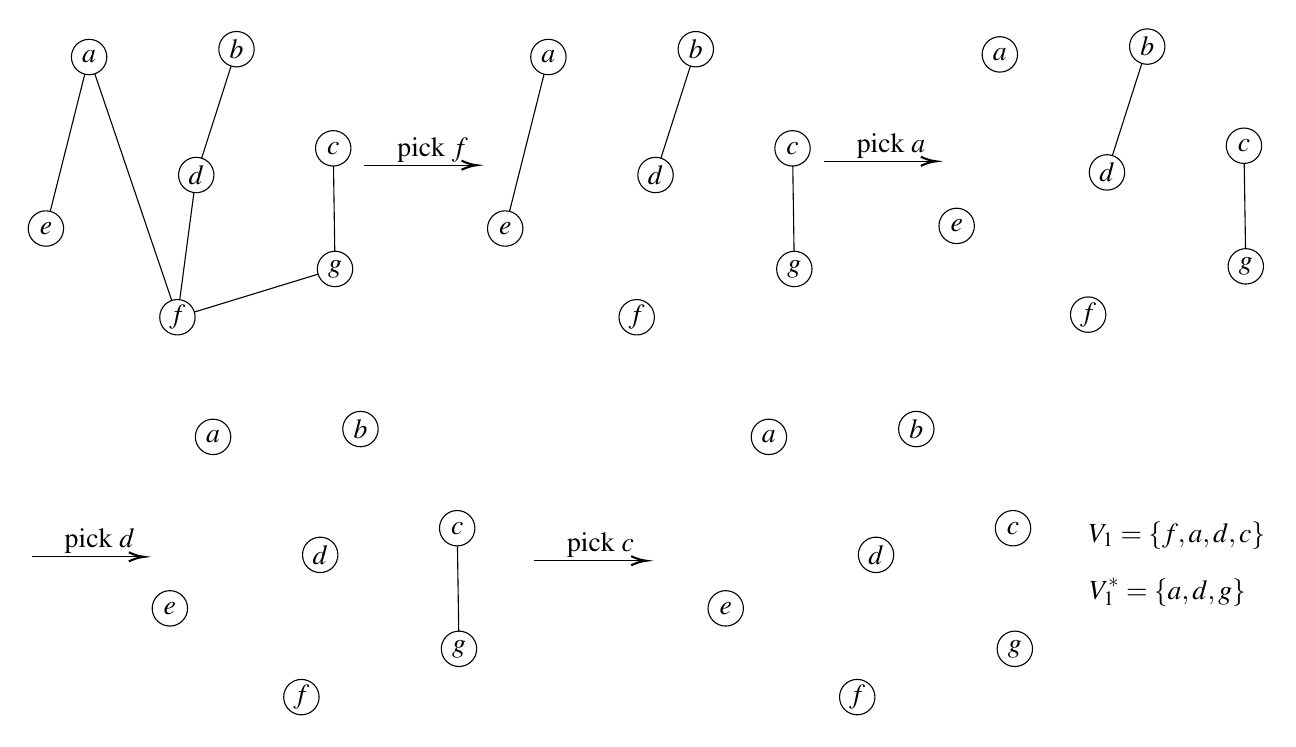
\begin{tikzpicture}[x=0.5pt,y=0.5pt,yscale=-1,xscale=1]
%uncomment if require: \path (0,509); %set diagram left start at 0, and has height of 509

%Straight Lines [id:da3853598268579197] 
\draw    (153.31,18.18) -- (124.22,109.11) ;
%Straight Lines [id:da21713072329995364] 
\draw    (224.52,177.01) -- (223.22,89.84) ;
%Straight Lines [id:da5478715757735835] 
\draw    (110.62,211.9) -- (224.52,177.01) ;
%Straight Lines [id:da42879006771456607] 
\draw    (46.79,23.83) -- (110.62,211.9) ;
%Straight Lines [id:da6771300098351073] 
\draw    (15.58,147.77) -- (46.79,23.83) ;
%Straight Lines [id:da4776548669152245] 
\draw    (110.62,211.9) -- (124.22,109.11) ;
%Shape: Ellipse [id:dp651117123053256] 
\draw  [fill={rgb, 255:red, 255; green, 255; blue, 255 }  ,fill opacity=1 ] (34,23.83) .. controls (34,16.77) and (39.73,11.04) .. (46.79,11.04) .. controls (53.86,11.04) and (59.58,16.77) .. (59.58,23.83) .. controls (59.58,30.9) and (53.86,36.62) .. (46.79,36.62) .. controls (39.73,36.62) and (34,30.9) .. (34,23.83) -- cycle ;
%Shape: Ellipse [id:dp7399561756845123] 
\draw  [fill={rgb, 255:red, 255; green, 255; blue, 255 }  ,fill opacity=1 ] (140.52,18.18) .. controls (140.52,11.11) and (146.25,5.39) .. (153.31,5.39) .. controls (160.38,5.39) and (166.1,11.11) .. (166.1,18.18) .. controls (166.1,25.24) and (160.38,30.97) .. (153.31,30.97) .. controls (146.25,30.97) and (140.52,25.24) .. (140.52,18.18) -- cycle ;
%Shape: Ellipse [id:dp8268258265249401] 
\draw  [fill={rgb, 255:red, 255; green, 255; blue, 255 }  ,fill opacity=1 ] (210.43,89.84) .. controls (210.43,82.78) and (216.15,77.05) .. (223.22,77.05) .. controls (230.28,77.05) and (236.01,82.78) .. (236.01,89.84) .. controls (236.01,96.9) and (230.28,102.63) .. (223.22,102.63) .. controls (216.15,102.63) and (210.43,96.9) .. (210.43,89.84) -- cycle ;
%Shape: Ellipse [id:dp5421818862330341] 
\draw  [fill={rgb, 255:red, 255; green, 255; blue, 255 }  ,fill opacity=1 ] (111.43,109.11) .. controls (111.43,102.05) and (117.15,96.32) .. (124.22,96.32) .. controls (131.28,96.32) and (137.01,102.05) .. (137.01,109.11) .. controls (137.01,116.18) and (131.28,121.9) .. (124.22,121.9) .. controls (117.15,121.9) and (111.43,116.18) .. (111.43,109.11) -- cycle ;
%Shape: Ellipse [id:dp45600813719389455] 
\draw  [fill={rgb, 255:red, 255; green, 255; blue, 255 }  ,fill opacity=1 ] (2.79,147.77) .. controls (2.79,140.71) and (8.52,134.98) .. (15.58,134.98) .. controls (22.64,134.98) and (28.37,140.71) .. (28.37,147.77) .. controls (28.37,154.84) and (22.64,160.56) .. (15.58,160.56) .. controls (8.52,160.56) and (2.79,154.84) .. (2.79,147.77) -- cycle ;
%Shape: Ellipse [id:dp031187496945339066] 
\draw  [fill={rgb, 255:red, 255; green, 255; blue, 255 }  ,fill opacity=1 ] (97.83,211.9) .. controls (97.83,204.83) and (103.56,199.11) .. (110.62,199.11) .. controls (117.69,199.11) and (123.41,204.83) .. (123.41,211.9) .. controls (123.41,218.96) and (117.69,224.69) .. (110.62,224.69) .. controls (103.56,224.69) and (97.83,218.96) .. (97.83,211.9) -- cycle ;
%Shape: Ellipse [id:dp7474313144054212] 
\draw  [fill={rgb, 255:red, 255; green, 255; blue, 255 }  ,fill opacity=1 ] (211.73,177.01) .. controls (211.73,169.94) and (217.46,164.22) .. (224.52,164.22) .. controls (231.59,164.22) and (237.31,169.94) .. (237.31,177.01) .. controls (237.31,184.07) and (231.59,189.8) .. (224.52,189.8) .. controls (217.46,189.8) and (211.73,184.07) .. (211.73,177.01) -- cycle ;
%Straight Lines [id:da10915523795701287] 
\draw    (485.24,18.18) -- (456.14,109.11) ;
%Straight Lines [id:da6013659372024278] 
\draw    (556.45,177.01) -- (555.14,89.84) ;
%Straight Lines [id:da2476997276246733] 
\draw    (347.5,147.77) -- (378.72,23.83) ;
%Shape: Ellipse [id:dp27040633021074256] 
\draw  [fill={rgb, 255:red, 255; green, 255; blue, 255 }  ,fill opacity=1 ] (365.93,23.83) .. controls (365.93,16.77) and (371.65,11.04) .. (378.72,11.04) .. controls (385.78,11.04) and (391.51,16.77) .. (391.51,23.83) .. controls (391.51,30.9) and (385.78,36.62) .. (378.72,36.62) .. controls (371.65,36.62) and (365.93,30.9) .. (365.93,23.83) -- cycle ;
%Shape: Ellipse [id:dp9153562797015269] 
\draw  [fill={rgb, 255:red, 255; green, 255; blue, 255 }  ,fill opacity=1 ] (472.45,18.18) .. controls (472.45,11.11) and (478.17,5.39) .. (485.24,5.39) .. controls (492.3,5.39) and (498.03,11.11) .. (498.03,18.18) .. controls (498.03,25.24) and (492.3,30.97) .. (485.24,30.97) .. controls (478.17,30.97) and (472.45,25.24) .. (472.45,18.18) -- cycle ;
%Shape: Ellipse [id:dp47379487417600374] 
\draw  [fill={rgb, 255:red, 255; green, 255; blue, 255 }  ,fill opacity=1 ] (542.35,89.84) .. controls (542.35,82.78) and (548.07,77.05) .. (555.14,77.05) .. controls (562.2,77.05) and (567.93,82.78) .. (567.93,89.84) .. controls (567.93,96.9) and (562.2,102.63) .. (555.14,102.63) .. controls (548.07,102.63) and (542.35,96.9) .. (542.35,89.84) -- cycle ;
%Shape: Ellipse [id:dp7207828118279439] 
\draw  [fill={rgb, 255:red, 255; green, 255; blue, 255 }  ,fill opacity=1 ] (443.35,109.11) .. controls (443.35,102.05) and (449.08,96.32) .. (456.14,96.32) .. controls (463.2,96.32) and (468.93,102.05) .. (468.93,109.11) .. controls (468.93,116.18) and (463.2,121.9) .. (456.14,121.9) .. controls (449.08,121.9) and (443.35,116.18) .. (443.35,109.11) -- cycle ;
%Shape: Ellipse [id:dp7155442322771159] 
\draw  [fill={rgb, 255:red, 255; green, 255; blue, 255 }  ,fill opacity=1 ] (334.71,147.77) .. controls (334.71,140.71) and (340.44,134.98) .. (347.5,134.98) .. controls (354.57,134.98) and (360.29,140.71) .. (360.29,147.77) .. controls (360.29,154.84) and (354.57,160.56) .. (347.5,160.56) .. controls (340.44,160.56) and (334.71,154.84) .. (334.71,147.77) -- cycle ;
%Shape: Ellipse [id:dp4818001756043101] 
\draw  [fill={rgb, 255:red, 255; green, 255; blue, 255 }  ,fill opacity=1 ] (429.75,211.9) .. controls (429.75,204.83) and (435.48,199.11) .. (442.54,199.11) .. controls (449.61,199.11) and (455.33,204.83) .. (455.33,211.9) .. controls (455.33,218.96) and (449.61,224.69) .. (442.54,224.69) .. controls (435.48,224.69) and (429.75,218.96) .. (429.75,211.9) -- cycle ;
%Shape: Ellipse [id:dp9764479331484588] 
\draw  [fill={rgb, 255:red, 255; green, 255; blue, 255 }  ,fill opacity=1 ] (543.66,177.01) .. controls (543.66,169.94) and (549.38,164.22) .. (556.45,164.22) .. controls (563.51,164.22) and (569.24,169.94) .. (569.24,177.01) .. controls (569.24,184.07) and (563.51,189.8) .. (556.45,189.8) .. controls (549.38,189.8) and (543.66,184.07) .. (543.66,177.01) -- cycle ;
%Straight Lines [id:da022074673171788572] 
\draw    (811.5,16.29) -- (782.4,107.23) ;
%Straight Lines [id:da7079754945425016] 
\draw    (882.71,175.12) -- (881.4,87.95) ;
%Shape: Ellipse [id:dp8120027238634924] 
\draw  [fill={rgb, 255:red, 255; green, 255; blue, 255 }  ,fill opacity=1 ] (692.19,21.95) .. controls (692.19,14.88) and (697.92,9.16) .. (704.98,9.16) .. controls (712.04,9.16) and (717.77,14.88) .. (717.77,21.95) .. controls (717.77,29.01) and (712.04,34.74) .. (704.98,34.74) .. controls (697.92,34.74) and (692.19,29.01) .. (692.19,21.95) -- cycle ;
%Shape: Ellipse [id:dp23465413123771173] 
\draw  [fill={rgb, 255:red, 255; green, 255; blue, 255 }  ,fill opacity=1 ] (798.71,16.29) .. controls (798.71,9.23) and (804.44,3.5) .. (811.5,3.5) .. controls (818.56,3.5) and (824.29,9.23) .. (824.29,16.29) .. controls (824.29,23.35) and (818.56,29.08) .. (811.5,29.08) .. controls (804.44,29.08) and (798.71,23.35) .. (798.71,16.29) -- cycle ;
%Shape: Ellipse [id:dp6697870946666823] 
\draw  [fill={rgb, 255:red, 255; green, 255; blue, 255 }  ,fill opacity=1 ] (868.61,87.95) .. controls (868.61,80.89) and (874.34,75.16) .. (881.4,75.16) .. controls (888.47,75.16) and (894.19,80.89) .. (894.19,87.95) .. controls (894.19,95.02) and (888.47,100.74) .. (881.4,100.74) .. controls (874.34,100.74) and (868.61,95.02) .. (868.61,87.95) -- cycle ;
%Shape: Ellipse [id:dp6678250120125151] 
\draw  [fill={rgb, 255:red, 255; green, 255; blue, 255 }  ,fill opacity=1 ] (769.61,107.23) .. controls (769.61,100.16) and (775.34,94.44) .. (782.4,94.44) .. controls (789.47,94.44) and (795.19,100.16) .. (795.19,107.23) .. controls (795.19,114.29) and (789.47,120.02) .. (782.4,120.02) .. controls (775.34,120.02) and (769.61,114.29) .. (769.61,107.23) -- cycle ;
%Shape: Ellipse [id:dp44880213332154095] 
\draw  [fill={rgb, 255:red, 255; green, 255; blue, 255 }  ,fill opacity=1 ] (660.98,145.89) .. controls (660.98,138.83) and (666.7,133.1) .. (673.77,133.1) .. controls (680.83,133.1) and (686.56,138.83) .. (686.56,145.89) .. controls (686.56,152.95) and (680.83,158.68) .. (673.77,158.68) .. controls (666.7,158.68) and (660.98,152.95) .. (660.98,145.89) -- cycle ;
%Shape: Ellipse [id:dp5261031453835676] 
\draw  [fill={rgb, 255:red, 255; green, 255; blue, 255 }  ,fill opacity=1 ] (756.02,210.01) .. controls (756.02,202.95) and (761.75,197.22) .. (768.81,197.22) .. controls (775.87,197.22) and (781.6,202.95) .. (781.6,210.01) .. controls (781.6,217.07) and (775.87,222.8) .. (768.81,222.8) .. controls (761.75,222.8) and (756.02,217.07) .. (756.02,210.01) -- cycle ;
%Shape: Ellipse [id:dp96264308088132] 
\draw  [fill={rgb, 255:red, 255; green, 255; blue, 255 }  ,fill opacity=1 ] (869.92,175.12) .. controls (869.92,168.06) and (875.65,162.33) .. (882.71,162.33) .. controls (889.77,162.33) and (895.5,168.06) .. (895.5,175.12) .. controls (895.5,182.18) and (889.77,187.91) .. (882.71,187.91) .. controls (875.65,187.91) and (869.92,182.18) .. (869.92,175.12) -- cycle ;
%Straight Lines [id:da5971152802941945] 
\draw    (314.1,451.53) -- (312.8,364.36) ;
%Shape: Ellipse [id:dp08371522903251905] 
\draw  [fill={rgb, 255:red, 255; green, 255; blue, 255 }  ,fill opacity=1 ] (123.58,298.35) .. controls (123.58,291.29) and (129.31,285.56) .. (136.37,285.56) .. controls (143.44,285.56) and (149.16,291.29) .. (149.16,298.35) .. controls (149.16,305.42) and (143.44,311.14) .. (136.37,311.14) .. controls (129.31,311.14) and (123.58,305.42) .. (123.58,298.35) -- cycle ;
%Shape: Ellipse [id:dp16754302978302682] 
\draw  [fill={rgb, 255:red, 255; green, 255; blue, 255 }  ,fill opacity=1 ] (230.11,292.7) .. controls (230.11,285.63) and (235.83,279.91) .. (242.9,279.91) .. controls (249.96,279.91) and (255.69,285.63) .. (255.69,292.7) .. controls (255.69,299.76) and (249.96,305.48) .. (242.9,305.48) .. controls (235.83,305.48) and (230.11,299.76) .. (230.11,292.7) -- cycle ;
%Shape: Ellipse [id:dp8803652600651565] 
\draw  [fill={rgb, 255:red, 255; green, 255; blue, 255 }  ,fill opacity=1 ] (300.01,364.36) .. controls (300.01,357.3) and (305.73,351.57) .. (312.8,351.57) .. controls (319.86,351.57) and (325.59,357.3) .. (325.59,364.36) .. controls (325.59,371.42) and (319.86,377.15) .. (312.8,377.15) .. controls (305.73,377.15) and (300.01,371.42) .. (300.01,364.36) -- cycle ;
%Shape: Ellipse [id:dp08434869719365379] 
\draw  [fill={rgb, 255:red, 255; green, 255; blue, 255 }  ,fill opacity=1 ] (201.01,383.63) .. controls (201.01,376.57) and (206.74,370.84) .. (213.8,370.84) .. controls (220.86,370.84) and (226.59,376.57) .. (226.59,383.63) .. controls (226.59,390.7) and (220.86,396.42) .. (213.8,396.42) .. controls (206.74,396.42) and (201.01,390.7) .. (201.01,383.63) -- cycle ;
%Shape: Ellipse [id:dp8697258636657205] 
\draw  [fill={rgb, 255:red, 255; green, 255; blue, 255 }  ,fill opacity=1 ] (92.37,422.29) .. controls (92.37,415.23) and (98.1,409.5) .. (105.16,409.5) .. controls (112.23,409.5) and (117.95,415.23) .. (117.95,422.29) .. controls (117.95,429.36) and (112.23,435.08) .. (105.16,435.08) .. controls (98.1,435.08) and (92.37,429.36) .. (92.37,422.29) -- cycle ;
%Shape: Ellipse [id:dp3796179832525568] 
\draw  [fill={rgb, 255:red, 255; green, 255; blue, 255 }  ,fill opacity=1 ] (187.41,486.42) .. controls (187.41,479.35) and (193.14,473.63) .. (200.2,473.63) .. controls (207.27,473.63) and (212.99,479.35) .. (212.99,486.42) .. controls (212.99,493.48) and (207.27,499.21) .. (200.2,499.21) .. controls (193.14,499.21) and (187.41,493.48) .. (187.41,486.42) -- cycle ;
%Shape: Ellipse [id:dp22651898621493904] 
\draw  [fill={rgb, 255:red, 255; green, 255; blue, 255 }  ,fill opacity=1 ] (301.32,451.53) .. controls (301.32,444.46) and (307.04,438.74) .. (314.1,438.74) .. controls (321.17,438.74) and (326.89,444.46) .. (326.89,451.53) .. controls (326.89,458.59) and (321.17,464.32) .. (314.1,464.32) .. controls (307.04,464.32) and (301.32,458.59) .. (301.32,451.53) -- cycle ;

%Shape: Ellipse [id:dp6886010266116899] 
\draw  [fill={rgb, 255:red, 255; green, 255; blue, 255 }  ,fill opacity=1 ] (525.29,298.35) .. controls (525.29,291.29) and (531.01,285.56) .. (538.08,285.56) .. controls (545.14,285.56) and (550.87,291.29) .. (550.87,298.35) .. controls (550.87,305.42) and (545.14,311.14) .. (538.08,311.14) .. controls (531.01,311.14) and (525.29,305.42) .. (525.29,298.35) -- cycle ;
%Shape: Ellipse [id:dp4406300893596924] 
\draw  [fill={rgb, 255:red, 255; green, 255; blue, 255 }  ,fill opacity=1 ] (631.81,292.7) .. controls (631.81,285.63) and (637.53,279.91) .. (644.6,279.91) .. controls (651.66,279.91) and (657.39,285.63) .. (657.39,292.7) .. controls (657.39,299.76) and (651.66,305.48) .. (644.6,305.48) .. controls (637.53,305.48) and (631.81,299.76) .. (631.81,292.7) -- cycle ;
%Shape: Ellipse [id:dp708253572812504] 
\draw  [fill={rgb, 255:red, 255; green, 255; blue, 255 }  ,fill opacity=1 ] (701.71,364.36) .. controls (701.71,357.3) and (707.43,351.57) .. (714.5,351.57) .. controls (721.56,351.57) and (727.29,357.3) .. (727.29,364.36) .. controls (727.29,371.42) and (721.56,377.15) .. (714.5,377.15) .. controls (707.43,377.15) and (701.71,371.42) .. (701.71,364.36) -- cycle ;
%Shape: Ellipse [id:dp12047908084857373] 
\draw  [fill={rgb, 255:red, 255; green, 255; blue, 255 }  ,fill opacity=1 ] (602.71,383.63) .. controls (602.71,376.57) and (608.44,370.84) .. (615.5,370.84) .. controls (622.56,370.84) and (628.29,376.57) .. (628.29,383.63) .. controls (628.29,390.7) and (622.56,396.42) .. (615.5,396.42) .. controls (608.44,396.42) and (602.71,390.7) .. (602.71,383.63) -- cycle ;
%Shape: Ellipse [id:dp06065835414250742] 
\draw  [fill={rgb, 255:red, 255; green, 255; blue, 255 }  ,fill opacity=1 ] (494.07,422.29) .. controls (494.07,415.23) and (499.8,409.5) .. (506.86,409.5) .. controls (513.93,409.5) and (519.65,415.23) .. (519.65,422.29) .. controls (519.65,429.36) and (513.93,435.08) .. (506.86,435.08) .. controls (499.8,435.08) and (494.07,429.36) .. (494.07,422.29) -- cycle ;
%Shape: Ellipse [id:dp7223087244252215] 
\draw  [fill={rgb, 255:red, 255; green, 255; blue, 255 }  ,fill opacity=1 ] (589.12,486.42) .. controls (589.12,479.35) and (594.84,473.63) .. (601.91,473.63) .. controls (608.97,473.63) and (614.69,479.35) .. (614.69,486.42) .. controls (614.69,493.48) and (608.97,499.21) .. (601.91,499.21) .. controls (594.84,499.21) and (589.12,493.48) .. (589.12,486.42) -- cycle ;
%Shape: Ellipse [id:dp483775428948783] 
\draw  [fill={rgb, 255:red, 255; green, 255; blue, 255 }  ,fill opacity=1 ] (703.02,451.53) .. controls (703.02,444.46) and (708.74,438.74) .. (715.81,438.74) .. controls (722.87,438.74) and (728.6,444.46) .. (728.6,451.53) .. controls (728.6,458.59) and (722.87,464.32) .. (715.81,464.32) .. controls (708.74,464.32) and (703.02,458.59) .. (703.02,451.53) -- cycle ;

%Straight Lines [id:da8565598108716722] 
\draw    (245.8,102.04) -- (324.89,102.04) ;
\draw [shift={(326.89,102.04)}, rotate = 180] [color={rgb, 255:red, 0; green, 0; blue, 0 }  ][line width=0.75]    (10.93,-3.29) .. controls (6.95,-1.4) and (3.31,-0.3) .. (0,0) .. controls (3.31,0.3) and (6.95,1.4) .. (10.93,3.29)   ;
%Straight Lines [id:da8466299980928367] 
\draw    (577.72,99.21) -- (656.82,99.21) ;
\draw [shift={(658.82,99.21)}, rotate = 180] [color={rgb, 255:red, 0; green, 0; blue, 0 }  ][line width=0.75]    (10.93,-3.29) .. controls (6.95,-1.4) and (3.31,-0.3) .. (0,0) .. controls (3.31,0.3) and (6.95,1.4) .. (10.93,3.29)   ;
%Straight Lines [id:da6943383967058451] 
\draw    (5.35,385.05) -- (84.44,385.05) ;
\draw [shift={(86.44,385.05)}, rotate = 180] [color={rgb, 255:red, 0; green, 0; blue, 0 }  ][line width=0.75]    (10.93,-3.29) .. controls (6.95,-1.4) and (3.31,-0.3) .. (0,0) .. controls (3.31,0.3) and (6.95,1.4) .. (10.93,3.29)   ;
%Straight Lines [id:da7622342093674817] 
\draw    (368.39,387.87) -- (447.48,387.87) ;
\draw [shift={(449.48,387.87)}, rotate = 180] [color={rgb, 255:red, 0; green, 0; blue, 0 }  ][line width=0.75]    (10.93,-3.29) .. controls (6.95,-1.4) and (3.31,-0.3) .. (0,0) .. controls (3.31,0.3) and (6.95,1.4) .. (10.93,3.29)   ;

% Text Node
\draw (767.36,358.13) node [anchor=north west][inner sep=0.75pt]   [align=left] {$\displaystyle V_{1} =\{f,a,d,c\}$};
% Text Node
\draw (767.82,398.59) node [anchor=north west][inner sep=0.75pt]   [align=left] {$\displaystyle V^{*}_{1} =\{a,d,g\}$};
% Text Node
\draw (46.79,23.83) node   [align=left] {$\displaystyle a$};
% Text Node
\draw (153.31,18.18) node   [align=left] {$\displaystyle b$};
% Text Node
\draw (223.22,89.84) node   [align=left] {$\displaystyle c$};
% Text Node
\draw (124.22,109.11) node   [align=left] {$\displaystyle d$};
% Text Node
\draw (15.58,147.77) node   [align=left] {$\displaystyle e$};
% Text Node
\draw (110.62,211.9) node   [align=left] {$\displaystyle f$};
% Text Node
\draw (224.52,177.01) node   [align=left] {$\displaystyle g$};
% Text Node
\draw (378.72,23.83) node   [align=left] {$\displaystyle a$};
% Text Node
\draw (485.24,18.18) node   [align=left] {$\displaystyle b$};
% Text Node
\draw (555.14,89.84) node   [align=left] {$\displaystyle c$};
% Text Node
\draw (456.14,109.11) node   [align=left] {$\displaystyle d$};
% Text Node
\draw (347.5,147.77) node   [align=left] {$\displaystyle e$};
% Text Node
\draw (442.54,211.9) node   [align=left] {$\displaystyle f$};
% Text Node
\draw (556.45,177.01) node   [align=left] {$\displaystyle g$};
% Text Node
\draw (704.98,21.95) node   [align=left] {$\displaystyle a$};
% Text Node
\draw (811.5,16.29) node   [align=left] {$\displaystyle b$};
% Text Node
\draw (881.4,87.95) node   [align=left] {$\displaystyle c$};
% Text Node
\draw (782.4,107.23) node   [align=left] {$\displaystyle d$};
% Text Node
\draw (673.77,145.89) node   [align=left] {$\displaystyle e$};
% Text Node
\draw (768.81,210.01) node   [align=left] {$\displaystyle f$};
% Text Node
\draw (882.71,175.12) node   [align=left] {$\displaystyle g$};
% Text Node
\draw (136.37,298.35) node   [align=left] {$\displaystyle a$};
% Text Node
\draw (242.9,292.7) node   [align=left] {$\displaystyle b$};
% Text Node
\draw (312.8,364.36) node   [align=left] {$\displaystyle c$};
% Text Node
\draw (213.8,383.63) node   [align=left] {$\displaystyle d$};
% Text Node
\draw (105.16,422.29) node   [align=left] {$\displaystyle e$};
% Text Node
\draw (200.2,486.42) node   [align=left] {$\displaystyle f$};
% Text Node
\draw (314.1,451.53) node   [align=left] {$\displaystyle g$};
% Text Node
\draw (538.08,298.35) node   [align=left] {$\displaystyle a$};
% Text Node
\draw (644.6,292.7) node   [align=left] {$\displaystyle b$};
% Text Node
\draw (714.5,364.36) node   [align=left] {$\displaystyle c$};
% Text Node
\draw (615.5,383.63) node   [align=left] {$\displaystyle d$};
% Text Node
\draw (506.86,422.29) node   [align=left] {$\displaystyle e$};
% Text Node
\draw (601.91,486.42) node   [align=left] {$\displaystyle f$};
% Text Node
\draw (715.81,451.53) node   [align=left] {$\displaystyle g$};
% Text Node
\draw (267.71,79.84) node [anchor=north west][inner sep=0.75pt]   [align=left] {pick $\displaystyle f$};
% Text Node
\draw (599.68,77.01) node [anchor=north west][inner sep=0.75pt]   [align=left] {pick $\displaystyle a$};
% Text Node
\draw (27.28,362.84) node [anchor=north west][inner sep=0.75pt]   [align=left] {pick $\displaystyle d$};
% Text Node
\draw (390.35,365.67) node [anchor=north west][inner sep=0.75pt]   [align=left] {pick $\displaystyle c$};


\end{tikzpicture}

}
\caption{Running above greedy algorithm on this instance:
	the picked vertex and the graph $(V, E_1)$
	in each iteration is illustrated. 
The greedy algorithm returns $V_1$, while the optimal solution is $V_1^*$.}
\label{fig:greedy1}
\end{figure}

\emph{Note: you may skip the following analysis and jump to the edge-based greedy algorithm.}
The performance of above algorithm could be very poor on certain instance.
Figure~\ref{fig:logn} gives such an instance, on which this algorithm
finds a vertex cover with $m\log m$ vertices, while the optimal solution
uses $m$ vertices. This instance is a \emph{bipartite graph}~(all vertices
are divided into two disjoint parts, and all edges are spanning the two parts;
the example shown in Figure~\ref{fig:greedy1} is a bipartite graph too; can you spot it?).
It's constructed as follows. The upper part consists of $m$ vertices.
The lower part consists of $m$ groups of vertices, and the $k$-th group
consists of $m/k$ vertices, $1\le k \le m$; 
each vertex in the $k$-th group connects to $k$ vertices
in the upper part, and two vertices in the $k$-th group
won't connect to the same vertex in the upper part.
Hence, every vertex in the upper part connects to a vertex in the $k$-th group once.
In the resulting graph, the degree of each vertex in the upper part is $m$,
and the degree of each vertex in the $k$-th group is $k$.

\begin{figure}[h]
\centering{

\tikzset{every picture/.style={line width=0.75pt}} %set default line width to 0.75pt        

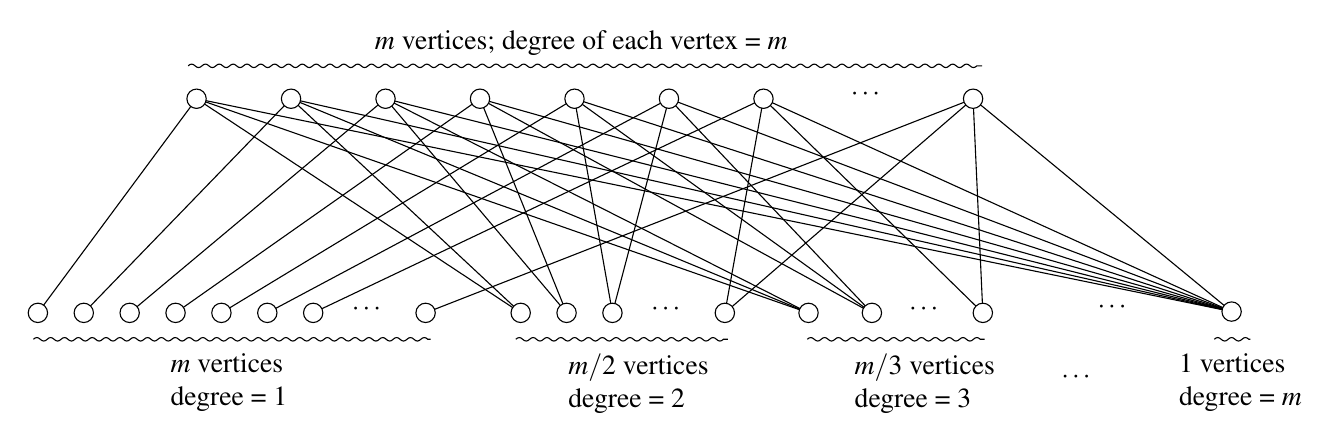
\begin{tikzpicture}[x=0.5pt,y=0.5pt,yscale=-1,xscale=1]
%uncomment if require: \path (0,301); %set diagram left start at 0, and has height of 301

%Straight Lines [id:da48256444006374477] 
\draw    (124.65,56.2) -- (9.99,210.95) ;
%Straight Lines [id:da7915530454104833] 
\draw    (192.94,56.2) -- (43.15,210.95) ;
%Straight Lines [id:da30042559203646113] 
\draw    (261.22,56.2) -- (76.31,210.95) ;
%Straight Lines [id:da9080822688714144] 
\draw    (329.5,56.2) -- (109.47,210.95) ;
%Straight Lines [id:da37114114846477] 
\draw    (397.79,56.2) -- (142.63,210.95) ;
%Straight Lines [id:da4658005175185246] 
\draw    (466.07,56.2) -- (175.78,210.95) ;
%Straight Lines [id:da5258947496178107] 
\draw    (534.36,56.2) -- (208.94,210.95) ;
%Straight Lines [id:da6645532958384183] 
\draw    (685.84,56.2) -- (290.17,210.95) ;
%Straight Lines [id:da10380018278005909] 
\draw    (124.65,56.2) -- (358.9,210.95) ;
%Straight Lines [id:da7761969194311258] 
\draw    (192.94,56.2) -- (358.9,210.95) ;
%Straight Lines [id:da5017214702936138] 
\draw    (261.22,56.2) -- (392.06,210.95) ;
%Straight Lines [id:da10567329008984383] 
\draw    (329.5,56.2) -- (392.06,210.95) ;
%Straight Lines [id:da44784285163898585] 
\draw    (397.79,56.2) -- (425.21,210.95) ;
%Straight Lines [id:da9254985226130398] 
\draw    (466.07,56.2) -- (425.21,210.95) ;
%Straight Lines [id:da6147419052612213] 
\draw    (534.36,56.2) -- (506.45,210.95) ;
%Straight Lines [id:da37997410936133735] 
\draw    (685.84,56.2) -- (506.45,210.95) ;
%Straight Lines [id:da3444361137026809] 
\draw    (124.65,56.2) -- (566.91,210.95) ;
%Straight Lines [id:da5994057734886903] 
\draw    (192.94,56.2) -- (566.91,210.95) ;
%Straight Lines [id:da5047286710832858] 
\draw    (261.22,56.2) -- (566.91,210.95) ;
%Straight Lines [id:da14316146210130398] 
\draw    (329.5,56.2) -- (612.72,210.95) ;
%Straight Lines [id:da2140446417746934] 
\draw    (397.79,56.2) -- (612.72,210.95) ;
%Straight Lines [id:da03146323129072537] 
\draw    (466.07,56.2) -- (612.72,210.95) ;
%Straight Lines [id:da5434407027169627] 
\draw    (534.36,56.2) -- (692.89,210.95) ;
%Straight Lines [id:da8329501485902712] 
\draw    (685.84,56.2) -- (692.89,210.95) ;
%Straight Lines [id:da4986567304461278] 
\draw    (124.65,56.2) -- (872.67,210.02) ;
%Straight Lines [id:da5196468578896155] 
\draw    (192.94,56.2) -- (872.67,210.02) ;
%Straight Lines [id:da27617247293660085] 
\draw    (261.22,56.2) -- (872.67,210.02) ;
%Straight Lines [id:da682030528339774] 
\draw    (329.5,56.2) -- (872.67,210.02) ;
%Straight Lines [id:da22339666198993757] 
\draw    (397.79,56.2) -- (872.67,210.02) ;
%Straight Lines [id:da95351562526954] 
\draw    (466.07,56.2) -- (872.67,210.02) ;
%Straight Lines [id:da9655555073242797] 
\draw    (534.36,56.2) -- (872.67,210.02) ;
%Straight Lines [id:da030869874243273587] 
\draw    (685.84,56.2) -- (872.67,210.02) ;
%Shape: Ellipse [id:dp9564687979886968] 
\draw  [fill={rgb, 255:red, 255; green, 255; blue, 255 }  ,fill opacity=1 ] (117.66,56.2) .. controls (117.66,52.34) and (120.79,49.21) .. (124.65,49.21) .. controls (128.51,49.21) and (131.64,52.34) .. (131.64,56.2) .. controls (131.64,60.06) and (128.51,63.19) .. (124.65,63.19) .. controls (120.79,63.19) and (117.66,60.06) .. (117.66,56.2) -- cycle ;
%Shape: Ellipse [id:dp15787288211587258] 
\draw  [fill={rgb, 255:red, 255; green, 255; blue, 255 }  ,fill opacity=1 ] (185.94,56.2) .. controls (185.94,52.34) and (189.08,49.21) .. (192.94,49.21) .. controls (196.8,49.21) and (199.93,52.34) .. (199.93,56.2) .. controls (199.93,60.06) and (196.8,63.19) .. (192.94,63.19) .. controls (189.08,63.19) and (185.94,60.06) .. (185.94,56.2) -- cycle ;
%Shape: Ellipse [id:dp31813541212711505] 
\draw  [fill={rgb, 255:red, 255; green, 255; blue, 255 }  ,fill opacity=1 ] (254.23,56.2) .. controls (254.23,52.34) and (257.36,49.21) .. (261.22,49.21) .. controls (265.08,49.21) and (268.21,52.34) .. (268.21,56.2) .. controls (268.21,60.06) and (265.08,63.19) .. (261.22,63.19) .. controls (257.36,63.19) and (254.23,60.06) .. (254.23,56.2) -- cycle ;
%Shape: Ellipse [id:dp6483512417570135] 
\draw  [fill={rgb, 255:red, 255; green, 255; blue, 255 }  ,fill opacity=1 ] (322.51,56.2) .. controls (322.51,52.34) and (325.64,49.21) .. (329.5,49.21) .. controls (333.37,49.21) and (336.5,52.34) .. (336.5,56.2) .. controls (336.5,60.06) and (333.37,63.19) .. (329.5,63.19) .. controls (325.64,63.19) and (322.51,60.06) .. (322.51,56.2) -- cycle ;
%Shape: Ellipse [id:dp005094034811534809] 
\draw  [fill={rgb, 255:red, 255; green, 255; blue, 255 }  ,fill opacity=1 ] (390.8,56.2) .. controls (390.8,52.34) and (393.93,49.21) .. (397.79,49.21) .. controls (401.65,49.21) and (404.78,52.34) .. (404.78,56.2) .. controls (404.78,60.06) and (401.65,63.19) .. (397.79,63.19) .. controls (393.93,63.19) and (390.8,60.06) .. (390.8,56.2) -- cycle ;
%Shape: Ellipse [id:dp1885467781241228] 
\draw  [fill={rgb, 255:red, 255; green, 255; blue, 255 }  ,fill opacity=1 ] (459.08,56.2) .. controls (459.08,52.34) and (462.21,49.21) .. (466.07,49.21) .. controls (469.93,49.21) and (473.06,52.34) .. (473.06,56.2) .. controls (473.06,60.06) and (469.93,63.19) .. (466.07,63.19) .. controls (462.21,63.19) and (459.08,60.06) .. (459.08,56.2) -- cycle ;
%Shape: Ellipse [id:dp9252145484504193] 
\draw  [fill={rgb, 255:red, 255; green, 255; blue, 255 }  ,fill opacity=1 ] (527.36,56.2) .. controls (527.36,52.34) and (530.49,49.21) .. (534.36,49.21) .. controls (538.22,49.21) and (541.35,52.34) .. (541.35,56.2) .. controls (541.35,60.06) and (538.22,63.19) .. (534.36,63.19) .. controls (530.49,63.19) and (527.36,60.06) .. (527.36,56.2) -- cycle ;
%Shape: Ellipse [id:dp1088055195079416] 
\draw  [fill={rgb, 255:red, 255; green, 255; blue, 255 }  ,fill opacity=1 ] (678.85,56.2) .. controls (678.85,52.34) and (681.98,49.21) .. (685.84,49.21) .. controls (689.7,49.21) and (692.83,52.34) .. (692.83,56.2) .. controls (692.83,60.06) and (689.7,63.19) .. (685.84,63.19) .. controls (681.98,63.19) and (678.85,60.06) .. (678.85,56.2) -- cycle ;
%Shape: Ellipse [id:dp805727227385243] 
\draw  [fill={rgb, 255:red, 255; green, 255; blue, 255 }  ,fill opacity=1 ] (3,210.95) .. controls (3,207.09) and (6.13,203.96) .. (9.99,203.96) .. controls (13.85,203.96) and (16.98,207.09) .. (16.98,210.95) .. controls (16.98,214.81) and (13.85,217.94) .. (9.99,217.94) .. controls (6.13,217.94) and (3,214.81) .. (3,210.95) -- cycle ;
%Shape: Ellipse [id:dp6927241755999763] 
\draw  [fill={rgb, 255:red, 255; green, 255; blue, 255 }  ,fill opacity=1 ] (69.32,210.95) .. controls (69.32,207.09) and (72.45,203.96) .. (76.31,203.96) .. controls (80.17,203.96) and (83.3,207.09) .. (83.3,210.95) .. controls (83.3,214.81) and (80.17,217.94) .. (76.31,217.94) .. controls (72.45,217.94) and (69.32,214.81) .. (69.32,210.95) -- cycle ;
%Shape: Ellipse [id:dp7140113684382683] 
\draw  [fill={rgb, 255:red, 255; green, 255; blue, 255 }  ,fill opacity=1 ] (135.63,210.95) .. controls (135.63,207.09) and (138.76,203.96) .. (142.63,203.96) .. controls (146.49,203.96) and (149.62,207.09) .. (149.62,210.95) .. controls (149.62,214.81) and (146.49,217.94) .. (142.63,217.94) .. controls (138.76,217.94) and (135.63,214.81) .. (135.63,210.95) -- cycle ;
%Shape: Circle [id:dp08051195272499023] 
\draw  [fill={rgb, 255:red, 255; green, 255; blue, 255 }  ,fill opacity=1 ] (168.79,210.95) .. controls (168.79,207.09) and (171.92,203.96) .. (175.78,203.96) .. controls (179.65,203.96) and (182.78,207.09) .. (182.78,210.95) .. controls (182.78,214.81) and (179.65,217.94) .. (175.78,217.94) .. controls (171.92,217.94) and (168.79,214.81) .. (168.79,210.95) -- cycle ;
%Shape: Circle [id:dp8836260613414209] 
\draw  [fill={rgb, 255:red, 255; green, 255; blue, 255 }  ,fill opacity=1 ] (283.18,210.95) .. controls (283.18,207.09) and (286.31,203.96) .. (290.17,203.96) .. controls (294.04,203.96) and (297.17,207.09) .. (297.17,210.95) .. controls (297.17,214.81) and (294.04,217.94) .. (290.17,217.94) .. controls (286.31,217.94) and (283.18,214.81) .. (283.18,210.95) -- cycle ;
%Shape: Ellipse [id:dp026005275946665574] 
\draw  [fill={rgb, 255:red, 255; green, 255; blue, 255 }  ,fill opacity=1 ] (201.95,210.95) .. controls (201.95,207.09) and (205.08,203.96) .. (208.94,203.96) .. controls (212.8,203.96) and (215.93,207.09) .. (215.93,210.95) .. controls (215.93,214.81) and (212.8,217.94) .. (208.94,217.94) .. controls (205.08,217.94) and (201.95,214.81) .. (201.95,210.95) -- cycle ;
%Shape: Ellipse [id:dp5514506286366462] 
\draw  [fill={rgb, 255:red, 255; green, 255; blue, 255 }  ,fill opacity=1 ] (102.48,210.95) .. controls (102.48,207.09) and (105.61,203.96) .. (109.47,203.96) .. controls (113.33,203.96) and (116.46,207.09) .. (116.46,210.95) .. controls (116.46,214.81) and (113.33,217.94) .. (109.47,217.94) .. controls (105.61,217.94) and (102.48,214.81) .. (102.48,210.95) -- cycle ;
%Shape: Ellipse [id:dp5878885517213746] 
\draw  [fill={rgb, 255:red, 255; green, 255; blue, 255 }  ,fill opacity=1 ] (36.16,210.95) .. controls (36.16,207.09) and (39.29,203.96) .. (43.15,203.96) .. controls (47.01,203.96) and (50.14,207.09) .. (50.14,210.95) .. controls (50.14,214.81) and (47.01,217.94) .. (43.15,217.94) .. controls (39.29,217.94) and (36.16,214.81) .. (36.16,210.95) -- cycle ;
%Shape: Circle [id:dp11688608679084533] 
\draw  [fill={rgb, 255:red, 255; green, 255; blue, 255 }  ,fill opacity=1 ] (351.91,210.95) .. controls (351.91,207.09) and (355.04,203.96) .. (358.9,203.96) .. controls (362.76,203.96) and (365.89,207.09) .. (365.89,210.95) .. controls (365.89,214.81) and (362.76,217.94) .. (358.9,217.94) .. controls (355.04,217.94) and (351.91,214.81) .. (351.91,210.95) -- cycle ;
%Shape: Ellipse [id:dp2691191844842149] 
\draw  [fill={rgb, 255:red, 255; green, 255; blue, 255 }  ,fill opacity=1 ] (385.06,210.95) .. controls (385.06,207.09) and (388.19,203.96) .. (392.06,203.96) .. controls (395.92,203.96) and (399.05,207.09) .. (399.05,210.95) .. controls (399.05,214.81) and (395.92,217.94) .. (392.06,217.94) .. controls (388.19,217.94) and (385.06,214.81) .. (385.06,210.95) -- cycle ;
%Shape: Ellipse [id:dp23564907218976294] 
\draw  [fill={rgb, 255:red, 255; green, 255; blue, 255 }  ,fill opacity=1 ] (499.45,210.95) .. controls (499.45,207.09) and (502.58,203.96) .. (506.45,203.96) .. controls (510.31,203.96) and (513.44,207.09) .. (513.44,210.95) .. controls (513.44,214.81) and (510.31,217.94) .. (506.45,217.94) .. controls (502.58,217.94) and (499.45,214.81) .. (499.45,210.95) -- cycle ;
%Shape: Circle [id:dp12095676578595771] 
\draw  [fill={rgb, 255:red, 255; green, 255; blue, 255 }  ,fill opacity=1 ] (418.22,210.95) .. controls (418.22,207.09) and (421.35,203.96) .. (425.21,203.96) .. controls (429.07,203.96) and (432.21,207.09) .. (432.21,210.95) .. controls (432.21,214.81) and (429.07,217.94) .. (425.21,217.94) .. controls (421.35,217.94) and (418.22,214.81) .. (418.22,210.95) -- cycle ;
%Straight Lines [id:da20103622480117145] 
\draw    (6.73,230.06) .. controls (8.4,228.39) and (10.06,228.39) .. (11.73,230.06) .. controls (13.4,231.73) and (15.06,231.73) .. (16.73,230.06) .. controls (18.4,228.39) and (20.06,228.39) .. (21.73,230.06) .. controls (23.4,231.73) and (25.06,231.73) .. (26.73,230.06) .. controls (28.4,228.39) and (30.06,228.39) .. (31.73,230.06) .. controls (33.4,231.73) and (35.06,231.73) .. (36.73,230.06) .. controls (38.4,228.39) and (40.06,228.39) .. (41.73,230.06) .. controls (43.4,231.73) and (45.06,231.73) .. (46.73,230.06) .. controls (48.4,228.39) and (50.06,228.39) .. (51.73,230.06) .. controls (53.4,231.73) and (55.06,231.73) .. (56.73,230.06) .. controls (58.4,228.39) and (60.06,228.39) .. (61.73,230.06) .. controls (63.4,231.73) and (65.06,231.73) .. (66.73,230.06) .. controls (68.4,228.39) and (70.06,228.39) .. (71.73,230.06) .. controls (73.4,231.73) and (75.06,231.73) .. (76.73,230.06) .. controls (78.4,228.39) and (80.06,228.39) .. (81.73,230.06) .. controls (83.4,231.73) and (85.06,231.73) .. (86.73,230.06) .. controls (88.4,228.39) and (90.06,228.39) .. (91.73,230.06) .. controls (93.4,231.73) and (95.06,231.73) .. (96.73,230.06) .. controls (98.4,228.39) and (100.06,228.39) .. (101.73,230.06) .. controls (103.4,231.73) and (105.06,231.73) .. (106.73,230.06) .. controls (108.4,228.39) and (110.06,228.39) .. (111.73,230.06) .. controls (113.4,231.73) and (115.06,231.73) .. (116.73,230.06) .. controls (118.4,228.39) and (120.06,228.39) .. (121.73,230.06) .. controls (123.4,231.73) and (125.06,231.73) .. (126.73,230.06) .. controls (128.4,228.39) and (130.06,228.39) .. (131.73,230.06) .. controls (133.4,231.73) and (135.06,231.73) .. (136.73,230.06) .. controls (138.4,228.39) and (140.06,228.39) .. (141.73,230.06) .. controls (143.4,231.73) and (145.06,231.73) .. (146.73,230.06) .. controls (148.4,228.39) and (150.06,228.39) .. (151.73,230.06) .. controls (153.4,231.73) and (155.06,231.73) .. (156.73,230.06) .. controls (158.4,228.39) and (160.06,228.39) .. (161.73,230.06) .. controls (163.4,231.73) and (165.06,231.73) .. (166.73,230.06) .. controls (168.4,228.39) and (170.06,228.39) .. (171.73,230.06) .. controls (173.4,231.73) and (175.06,231.73) .. (176.73,230.06) .. controls (178.4,228.39) and (180.06,228.39) .. (181.73,230.06) .. controls (183.4,231.73) and (185.06,231.73) .. (186.73,230.06) .. controls (188.4,228.39) and (190.06,228.39) .. (191.73,230.06) .. controls (193.4,231.73) and (195.06,231.73) .. (196.73,230.06) .. controls (198.4,228.39) and (200.06,228.39) .. (201.73,230.06) .. controls (203.4,231.73) and (205.06,231.73) .. (206.73,230.06) .. controls (208.4,228.39) and (210.06,228.39) .. (211.73,230.06) .. controls (213.4,231.73) and (215.06,231.73) .. (216.73,230.06) .. controls (218.4,228.39) and (220.06,228.39) .. (221.73,230.06) .. controls (223.4,231.73) and (225.06,231.73) .. (226.73,230.06) .. controls (228.4,228.39) and (230.06,228.39) .. (231.73,230.06) .. controls (233.4,231.73) and (235.06,231.73) .. (236.73,230.06) .. controls (238.4,228.39) and (240.06,228.39) .. (241.73,230.06) .. controls (243.4,231.73) and (245.06,231.73) .. (246.73,230.06) .. controls (248.4,228.39) and (250.06,228.39) .. (251.73,230.06) .. controls (253.4,231.73) and (255.06,231.73) .. (256.73,230.06) .. controls (258.4,228.39) and (260.06,228.39) .. (261.73,230.06) .. controls (263.4,231.73) and (265.06,231.73) .. (266.73,230.06) .. controls (268.4,228.39) and (270.06,228.39) .. (271.73,230.06) .. controls (273.4,231.73) and (275.06,231.73) .. (276.73,230.06) .. controls (278.4,228.39) and (280.06,228.39) .. (281.73,230.06) .. controls (283.4,231.73) and (285.06,231.73) .. (286.73,230.06) .. controls (288.4,228.39) and (290.06,228.39) .. (291.73,230.06) -- (293.85,230.06) -- (293.85,230.06) ;
%Shape: Ellipse [id:dp8464809367337334] 
\draw  [fill={rgb, 255:red, 255; green, 255; blue, 255 }  ,fill opacity=1 ] (685.89,210.95) .. controls (685.89,207.09) and (689.03,203.96) .. (692.89,203.96) .. controls (696.75,203.96) and (699.88,207.09) .. (699.88,210.95) .. controls (699.88,214.81) and (696.75,217.94) .. (692.89,217.94) .. controls (689.03,217.94) and (685.89,214.81) .. (685.89,210.95) -- cycle ;
%Shape: Ellipse [id:dp65977848187328] 
\draw  [fill={rgb, 255:red, 255; green, 255; blue, 255 }  ,fill opacity=1 ] (559.92,210.95) .. controls (559.92,207.09) and (563.05,203.96) .. (566.91,203.96) .. controls (570.77,203.96) and (573.9,207.09) .. (573.9,210.95) .. controls (573.9,214.81) and (570.77,217.94) .. (566.91,217.94) .. controls (563.05,217.94) and (559.92,214.81) .. (559.92,210.95) -- cycle ;
%Shape: Ellipse [id:dp16067413663955887] 
\draw  [fill={rgb, 255:red, 255; green, 255; blue, 255 }  ,fill opacity=1 ] (865.68,210.02) .. controls (865.68,206.16) and (868.81,203.03) .. (872.67,203.03) .. controls (876.53,203.03) and (879.66,206.16) .. (879.66,210.02) .. controls (879.66,213.88) and (876.53,217.01) .. (872.67,217.01) .. controls (868.81,217.01) and (865.68,213.88) .. (865.68,210.02) -- cycle ;
%Shape: Ellipse [id:dp49168873794934076] 
\draw  [fill={rgb, 255:red, 255; green, 255; blue, 255 }  ,fill opacity=1 ] (605.73,210.95) .. controls (605.73,207.09) and (608.86,203.96) .. (612.72,203.96) .. controls (616.58,203.96) and (619.71,207.09) .. (619.71,210.95) .. controls (619.71,214.81) and (616.58,217.94) .. (612.72,217.94) .. controls (608.86,217.94) and (605.73,214.81) .. (605.73,210.95) -- cycle ;
%Straight Lines [id:da15506183031027287] 
\draw    (355.37,230.06) .. controls (357.04,228.39) and (358.7,228.39) .. (360.37,230.06) .. controls (362.04,231.73) and (363.7,231.73) .. (365.37,230.06) .. controls (367.04,228.39) and (368.7,228.39) .. (370.37,230.06) .. controls (372.04,231.73) and (373.7,231.73) .. (375.37,230.06) .. controls (377.04,228.39) and (378.7,228.39) .. (380.37,230.06) .. controls (382.04,231.73) and (383.7,231.73) .. (385.37,230.06) .. controls (387.04,228.39) and (388.7,228.39) .. (390.37,230.06) .. controls (392.04,231.73) and (393.7,231.73) .. (395.37,230.06) .. controls (397.04,228.39) and (398.7,228.39) .. (400.37,230.06) .. controls (402.04,231.73) and (403.7,231.73) .. (405.37,230.06) .. controls (407.04,228.39) and (408.7,228.39) .. (410.37,230.06) .. controls (412.04,231.73) and (413.7,231.73) .. (415.37,230.06) .. controls (417.04,228.39) and (418.7,228.39) .. (420.37,230.06) .. controls (422.04,231.73) and (423.7,231.73) .. (425.37,230.06) .. controls (427.04,228.39) and (428.7,228.39) .. (430.37,230.06) .. controls (432.04,231.73) and (433.7,231.73) .. (435.37,230.06) .. controls (437.04,228.39) and (438.7,228.39) .. (440.37,230.06) .. controls (442.04,231.73) and (443.7,231.73) .. (445.37,230.06) .. controls (447.04,228.39) and (448.7,228.39) .. (450.37,230.06) .. controls (452.04,231.73) and (453.7,231.73) .. (455.37,230.06) .. controls (457.04,228.39) and (458.7,228.39) .. (460.37,230.06) .. controls (462.04,231.73) and (463.7,231.73) .. (465.37,230.06) .. controls (467.04,228.39) and (468.7,228.39) .. (470.37,230.06) .. controls (472.04,231.73) and (473.7,231.73) .. (475.37,230.06) .. controls (477.04,228.39) and (478.7,228.39) .. (480.37,230.06) .. controls (482.04,231.73) and (483.7,231.73) .. (485.37,230.06) .. controls (487.04,228.39) and (488.7,228.39) .. (490.37,230.06) .. controls (492.04,231.73) and (493.7,231.73) .. (495.37,230.06) .. controls (497.04,228.39) and (498.7,228.39) .. (500.37,230.06) .. controls (502.04,231.73) and (503.7,231.73) .. (505.37,230.06) -- (508.72,230.06) -- (508.72,230.06) ;
%Straight Lines [id:da43523296367867814] 
\draw    (566.05,230.06) .. controls (567.72,228.39) and (569.38,228.39) .. (571.05,230.06) .. controls (572.72,231.73) and (574.38,231.73) .. (576.05,230.06) .. controls (577.72,228.39) and (579.38,228.39) .. (581.05,230.06) .. controls (582.72,231.73) and (584.38,231.73) .. (586.05,230.06) .. controls (587.72,228.39) and (589.38,228.39) .. (591.05,230.06) .. controls (592.72,231.73) and (594.38,231.73) .. (596.05,230.06) .. controls (597.72,228.39) and (599.38,228.39) .. (601.05,230.06) .. controls (602.72,231.73) and (604.38,231.73) .. (606.05,230.06) .. controls (607.72,228.39) and (609.38,228.39) .. (611.05,230.06) .. controls (612.72,231.73) and (614.38,231.73) .. (616.05,230.06) .. controls (617.72,228.39) and (619.38,228.39) .. (621.05,230.06) .. controls (622.72,231.73) and (624.38,231.73) .. (626.05,230.06) .. controls (627.72,228.39) and (629.38,228.39) .. (631.05,230.06) .. controls (632.72,231.73) and (634.38,231.73) .. (636.05,230.06) .. controls (637.72,228.39) and (639.38,228.39) .. (641.05,230.06) .. controls (642.72,231.73) and (644.38,231.73) .. (646.05,230.06) .. controls (647.72,228.39) and (649.38,228.39) .. (651.05,230.06) .. controls (652.72,231.73) and (654.38,231.73) .. (656.05,230.06) .. controls (657.72,228.39) and (659.38,228.39) .. (661.05,230.06) .. controls (662.72,231.73) and (664.38,231.73) .. (666.05,230.06) .. controls (667.72,228.39) and (669.38,228.39) .. (671.05,230.06) .. controls (672.72,231.73) and (674.38,231.73) .. (676.05,230.06) .. controls (677.72,228.39) and (679.38,228.39) .. (681.05,230.06) .. controls (682.72,231.73) and (684.38,231.73) .. (686.05,230.06) .. controls (687.72,228.39) and (689.38,228.39) .. (691.05,230.06) -- (694.23,230.06) -- (694.23,230.06) ;
%Straight Lines [id:da28592023171431014] 
\draw    (860.16,230.06) .. controls (861.83,228.39) and (863.49,228.39) .. (865.16,230.06) .. controls (866.83,231.73) and (868.49,231.73) .. (870.16,230.06) .. controls (871.83,228.39) and (873.49,228.39) .. (875.16,230.06) .. controls (876.83,231.73) and (878.49,231.73) .. (880.16,230.06) .. controls (881.83,228.39) and (883.49,228.39) .. (885.16,230.06) -- (886.26,230.06) -- (886.26,230.06) ;
%Straight Lines [id:da9947827870575903] 
\draw    (118.59,32.43) .. controls (120.26,30.76) and (121.92,30.76) .. (123.59,32.43) .. controls (125.26,34.1) and (126.92,34.1) .. (128.59,32.43) .. controls (130.26,30.76) and (131.92,30.76) .. (133.59,32.43) .. controls (135.26,34.1) and (136.92,34.1) .. (138.59,32.43) .. controls (140.26,30.76) and (141.92,30.76) .. (143.59,32.43) .. controls (145.26,34.1) and (146.92,34.1) .. (148.59,32.43) .. controls (150.26,30.76) and (151.92,30.76) .. (153.59,32.43) .. controls (155.26,34.1) and (156.92,34.1) .. (158.59,32.43) .. controls (160.26,30.76) and (161.92,30.76) .. (163.59,32.43) .. controls (165.26,34.1) and (166.92,34.1) .. (168.59,32.43) .. controls (170.26,30.76) and (171.92,30.76) .. (173.59,32.43) .. controls (175.26,34.1) and (176.92,34.1) .. (178.59,32.43) .. controls (180.26,30.76) and (181.92,30.76) .. (183.59,32.43) .. controls (185.26,34.1) and (186.92,34.1) .. (188.59,32.43) .. controls (190.26,30.76) and (191.92,30.76) .. (193.59,32.43) .. controls (195.26,34.1) and (196.92,34.1) .. (198.59,32.43) .. controls (200.26,30.76) and (201.92,30.76) .. (203.59,32.43) .. controls (205.26,34.1) and (206.92,34.1) .. (208.59,32.43) .. controls (210.26,30.76) and (211.92,30.76) .. (213.59,32.43) .. controls (215.26,34.1) and (216.92,34.1) .. (218.59,32.43) .. controls (220.26,30.76) and (221.92,30.76) .. (223.59,32.43) .. controls (225.26,34.1) and (226.92,34.1) .. (228.59,32.43) .. controls (230.26,30.76) and (231.92,30.76) .. (233.59,32.43) .. controls (235.26,34.1) and (236.92,34.1) .. (238.59,32.43) .. controls (240.26,30.76) and (241.92,30.76) .. (243.59,32.43) .. controls (245.26,34.1) and (246.92,34.1) .. (248.59,32.43) .. controls (250.26,30.76) and (251.92,30.76) .. (253.59,32.43) .. controls (255.26,34.1) and (256.92,34.1) .. (258.59,32.43) .. controls (260.26,30.76) and (261.92,30.76) .. (263.59,32.43) .. controls (265.26,34.1) and (266.92,34.1) .. (268.59,32.43) .. controls (270.26,30.76) and (271.92,30.76) .. (273.59,32.43) .. controls (275.26,34.1) and (276.92,34.1) .. (278.59,32.43) .. controls (280.26,30.76) and (281.92,30.76) .. (283.59,32.43) .. controls (285.26,34.1) and (286.92,34.1) .. (288.59,32.43) .. controls (290.26,30.76) and (291.92,30.76) .. (293.59,32.43) .. controls (295.26,34.1) and (296.92,34.1) .. (298.59,32.43) .. controls (300.26,30.76) and (301.92,30.76) .. (303.59,32.43) .. controls (305.26,34.1) and (306.92,34.1) .. (308.59,32.43) .. controls (310.26,30.76) and (311.92,30.76) .. (313.59,32.43) .. controls (315.26,34.1) and (316.92,34.1) .. (318.59,32.43) .. controls (320.26,30.76) and (321.92,30.76) .. (323.59,32.43) .. controls (325.26,34.1) and (326.92,34.1) .. (328.59,32.43) .. controls (330.26,30.76) and (331.92,30.76) .. (333.59,32.43) .. controls (335.26,34.1) and (336.92,34.1) .. (338.59,32.43) .. controls (340.26,30.76) and (341.92,30.76) .. (343.59,32.43) .. controls (345.26,34.1) and (346.92,34.1) .. (348.59,32.43) .. controls (350.26,30.76) and (351.92,30.76) .. (353.59,32.43) .. controls (355.26,34.1) and (356.92,34.1) .. (358.59,32.43) .. controls (360.26,30.76) and (361.92,30.76) .. (363.59,32.43) .. controls (365.26,34.1) and (366.92,34.1) .. (368.59,32.43) .. controls (370.26,30.76) and (371.92,30.76) .. (373.59,32.43) .. controls (375.26,34.1) and (376.92,34.1) .. (378.59,32.43) .. controls (380.26,30.76) and (381.92,30.76) .. (383.59,32.43) .. controls (385.26,34.1) and (386.92,34.1) .. (388.59,32.43) .. controls (390.26,30.76) and (391.92,30.76) .. (393.59,32.43) .. controls (395.26,34.1) and (396.92,34.1) .. (398.59,32.43) .. controls (400.26,30.76) and (401.92,30.76) .. (403.59,32.43) .. controls (405.26,34.1) and (406.92,34.1) .. (408.59,32.43) .. controls (410.26,30.76) and (411.92,30.76) .. (413.59,32.43) .. controls (415.26,34.1) and (416.92,34.1) .. (418.59,32.43) .. controls (420.26,30.76) and (421.92,30.76) .. (423.59,32.43) .. controls (425.26,34.1) and (426.92,34.1) .. (428.59,32.43) .. controls (430.26,30.76) and (431.92,30.76) .. (433.59,32.43) .. controls (435.26,34.1) and (436.92,34.1) .. (438.59,32.43) .. controls (440.26,30.76) and (441.92,30.76) .. (443.59,32.43) .. controls (445.26,34.1) and (446.92,34.1) .. (448.59,32.43) .. controls (450.26,30.76) and (451.92,30.76) .. (453.59,32.43) .. controls (455.26,34.1) and (456.92,34.1) .. (458.59,32.43) .. controls (460.26,30.76) and (461.92,30.76) .. (463.59,32.43) .. controls (465.26,34.1) and (466.92,34.1) .. (468.59,32.43) .. controls (470.26,30.76) and (471.92,30.76) .. (473.59,32.43) .. controls (475.26,34.1) and (476.92,34.1) .. (478.59,32.43) .. controls (480.26,30.76) and (481.92,30.76) .. (483.59,32.43) .. controls (485.26,34.1) and (486.92,34.1) .. (488.59,32.43) .. controls (490.26,30.76) and (491.92,30.76) .. (493.59,32.43) .. controls (495.26,34.1) and (496.92,34.1) .. (498.59,32.43) .. controls (500.26,30.76) and (501.92,30.76) .. (503.59,32.43) .. controls (505.26,34.1) and (506.92,34.1) .. (508.59,32.43) .. controls (510.26,30.76) and (511.92,30.76) .. (513.59,32.43) .. controls (515.26,34.1) and (516.92,34.1) .. (518.59,32.43) .. controls (520.26,30.76) and (521.92,30.76) .. (523.59,32.43) .. controls (525.26,34.1) and (526.92,34.1) .. (528.59,32.43) .. controls (530.26,30.76) and (531.92,30.76) .. (533.59,32.43) .. controls (535.26,34.1) and (536.92,34.1) .. (538.59,32.43) .. controls (540.26,30.76) and (541.92,30.76) .. (543.59,32.43) .. controls (545.26,34.1) and (546.92,34.1) .. (548.59,32.43) .. controls (550.26,30.76) and (551.92,30.76) .. (553.59,32.43) .. controls (555.26,34.1) and (556.92,34.1) .. (558.59,32.43) .. controls (560.26,30.76) and (561.92,30.76) .. (563.59,32.43) .. controls (565.26,34.1) and (566.92,34.1) .. (568.59,32.43) .. controls (570.26,30.76) and (571.92,30.76) .. (573.59,32.43) .. controls (575.26,34.1) and (576.92,34.1) .. (578.59,32.43) .. controls (580.26,30.76) and (581.92,30.76) .. (583.59,32.43) .. controls (585.26,34.1) and (586.92,34.1) .. (588.59,32.43) .. controls (590.26,30.76) and (591.92,30.76) .. (593.59,32.43) .. controls (595.26,34.1) and (596.92,34.1) .. (598.59,32.43) .. controls (600.26,30.76) and (601.92,30.76) .. (603.59,32.43) .. controls (605.26,34.1) and (606.92,34.1) .. (608.59,32.43) .. controls (610.26,30.76) and (611.92,30.76) .. (613.59,32.43) .. controls (615.26,34.1) and (616.92,34.1) .. (618.59,32.43) .. controls (620.26,30.76) and (621.92,30.76) .. (623.59,32.43) .. controls (625.26,34.1) and (626.92,34.1) .. (628.59,32.43) .. controls (630.26,30.76) and (631.92,30.76) .. (633.59,32.43) .. controls (635.26,34.1) and (636.92,34.1) .. (638.59,32.43) .. controls (640.26,30.76) and (641.92,30.76) .. (643.59,32.43) .. controls (645.26,34.1) and (646.92,34.1) .. (648.59,32.43) .. controls (650.26,30.76) and (651.92,30.76) .. (653.59,32.43) .. controls (655.26,34.1) and (656.92,34.1) .. (658.59,32.43) .. controls (660.26,30.76) and (661.92,30.76) .. (663.59,32.43) .. controls (665.26,34.1) and (666.92,34.1) .. (668.59,32.43) .. controls (670.26,30.76) and (671.92,30.76) .. (673.59,32.43) .. controls (675.26,34.1) and (676.92,34.1) .. (678.59,32.43) .. controls (680.26,30.76) and (681.92,30.76) .. (683.59,32.43) .. controls (685.26,34.1) and (686.92,34.1) .. (688.59,32.43) -- (692.36,32.43) -- (692.36,32.43) ;

% Text Node
\draw (595.6,47.2) node [anchor=north west][inner sep=0.75pt]   [align=left] {$\displaystyle \cdots $};
% Text Node
\draw (235.06,201.95) node [anchor=north west][inner sep=0.75pt]   [align=left] {$\displaystyle \cdots $};
% Text Node
\draw (451.33,201.95) node [anchor=north west][inner sep=0.75pt]   [align=left] {$\displaystyle \cdots $};
% Text Node
\draw (637.77,202.42) node [anchor=north west][inner sep=0.75pt]   [align=left] {$\displaystyle \cdots $};
% Text Node
\draw (773.87,201.02) node [anchor=north west][inner sep=0.75pt]   [align=left] {$\displaystyle \cdots $};
% Text Node
\draw (103.97,238.49) node [anchor=north west][inner sep=0.75pt]   [align=left] {$\displaystyle m$ vertices\\degree = $\displaystyle 1$};
% Text Node
\draw (391.44,238.49) node [anchor=north west][inner sep=0.75pt]   [align=left] {$\displaystyle m/2$ vertices\\degree = $\displaystyle 2$};
% Text Node
\draw (598.39,238.49) node [anchor=north west][inner sep=0.75pt]   [align=left] {$\displaystyle m/3$ vertices\\degree = $\displaystyle 3$};
% Text Node
\draw (832.78,238.49) node [anchor=north west][inner sep=0.75pt]   [align=left] {$\displaystyle 1$ vertices\\degree = $\displaystyle m$};
% Text Node
\draw (251.64,5.25) node [anchor=north west][inner sep=0.75pt]   [align=left] {$\displaystyle m$ vertices; degree of each vertex = $\displaystyle m$};
% Text Node
\draw (747.77,251.36) node [anchor=north west][inner sep=0.75pt]   [align=left] {$\displaystyle \cdots $};


\end{tikzpicture}

}
\caption{An instance on which above vertex-based approximation 
algorithm finds a vertex cover consists of all vertices in the
lower part, while the optimal solution consists of all vertices
in the upper part.}
\label{fig:logn}
\end{figure}

Let's run above greedy algorithm on this complex instance.
Recall that the algorithm picks the vertex with largest degree in
each iteration. %assuming that the graph will be kept updated by removing these edges that are covered by the picked vertex in each iteration. 
Consider the first iteration, 
these $m$ vertices in the upper part and the $m$-th group in the lower part~(with 1 vertex)
all have the largest degree of $m$.
At a bad luck the algorithm picks the one in the lower part.
After removing its adjacent edges, the vertices in the upper part
have degree of $(m-1)$.
Consider the second iteration,
again the $m$ vertices in the upper part and the $(m-1)$-th group in the lower part~(with $\lfloor m/(m-1) \rfloor$ vertices)
have degree of $(m-1)$.
And assume that the algorithm picks the one(s) in the lower part.
Clearly, if the algorithm always picks the vertices in the lower part
to break tie, the solution returned by this greedy algorithm will include all vertices in the lower part: the total
number of vertices is $m + m/2 + m/3 + \cdots + m/m = \Theta(m\log m)$.
Notice that the optimal solution consists of all vertices in the upper part with $m$ vertices.
Hence, the ratio on this instance is $\Theta(m\log m / m) = \Theta(\log m)$.

Is above complex instance the worst-case example for this greedy algorithm~(i.e.,
the ratio is maximized among all instances)?
Actually yes~(in asymptotic manner).
Formally, we can prove that, the ratio is bounded by $\Theta(\log |E|)$. In
other words, this algorithm is an \emph{approximation algorithm} with an approximation
ratio of $\Theta(\log |E|)$.
\begin{fact}
Let $V_1$ be the vertex cover returned by above (vertex-based) greedy algorithm.
Let $V_1^*$ be the optimal vertex cover.
We have $|V_1| \le \Theta(\log |E|) |V_1^*|$.
\end{fact}
\emph{Proof.}
Assume that $|V_1| = k$ and $|V_1^*| = k^*$.
Assume that the greedy algorithm iteratively picks $v_1, v_2, \cdots, v_k$,
and assume that in the beginning of the $i$-th iteration, the degree of $v_i$ is $m_i$.  We have the following facts.
\vspace*{-\topsep}
\begin{enumerate}
\item After the $i$-th iteration~(or before the $(i+1)$-th iteration),
there are $|E| - \sum_{j=1}^i m_j$ edges in the graph,
as $m_i$ edges will be removed in the $i$-th iteration.
\item In the beginning of the $i$-th iteration,
there are $|E| - \sum_{j=1}^{i-1} m_j$ edges in the graph.
Let $d(v)$ be the degree of $v$ at this time. 
Recall that $V_1^*$ is a cover, i.e., $|V_1^*|$ covers all edges~(at any time of the algorithm). 
Hence, we have $\sum_{v\in V_1^*} d(v) \ge |E| - \sum_{j=1}^{i-1} m_j$.
\item Since the greedy algorithm always picks the vertex
with the largest degree in each iteration, we know that $m_i$ is the largest 
degree in the graph in the beginning of the $i$-th iteration.
Combined with above item, we can write $|E| - \sum_{j=1}^{i-1} m_j \le \sum_{v\in V_1^*} d(v) \le \sum_{v\in V_1^*} m_i = m_i \cdot k^*$.
\end{enumerate}

We therefore have $|E| - \sum_{j=1}^{i-1} m_j \le  m_i \cdot k^*$, for any $1\le i \le k$.
We now use it to bound $m_i$ and $|E| - \sum_{j=1}^{i} m_j$, i.e., the number of edges remaining after $i$-th iteration. 
\vspace*{-\topsep}
\begin{enumerate}
\item For $i = 1$, $|E| \le m_1 \cdot k^*$ and therefore $m_1 \ge |E| / k^*$.
Hence $|E| - m_1 \le |E| - |E|/k^* = |E| \cdot (1-1/k^*)$.

\item For $i = 2$, $|E| - m_1 \le m_2 \cdot k^*$ and therefore $m_2 \ge (|E| - m_1) / k^*$.
Hence $|E| - m_1 - m_2 \le |E| - m_1 - (|E| - m_1)/k^* = (|E| - m_1) \cdot (1-1/k^*) \le |E|\cdot(1-1/k^*)^2$.

\item For $i = 3$, $|E| - m_1 - m_2 \le m_3 \cdot k^*$ and therefore $m_3 \ge (|E| - m_1 - m_2) / k^*$.
Hence $|E| - m_1 - m_2 - m_3\le |E| - m_1 - m_2 - (|E| - m_1 - m_2)/k^* = (|E| - m_1 - m_2) \cdot (1-1/k^*) \le |E|\cdot(1-1/k^*)^3$.
\end{enumerate}

Clearly, after $k-1$ iterations, 
we have $|E| - \sum_{j=1}^{k-1} m_i \le |E| \cdot (1-1/k^*)^{k-1}$.
Note that at this time the graph contains $m_k$ edges and $m_k \ge 1$.
Hence, we have $|E| \cdot (1-1/k^*)^{k-1} \ge 1$.
Take $\log(\cdot)$ on both sides, we have $\log |E| + (k-1)\cdot \log (1-1/k^*) \ge 0$.

We apply $(1+x)\le e^x$ with $x = -1/k^*$.
We have $0 \le \log |E| + (k-1)\cdot \log (1-1/k^*) \le \log |E| - (k-1)/k^*$.
This gives $(k-1)/k^* \le \log |E|$, and also implies 
$k/k^* \le \Theta(\log |E|)$, a desired result. \qed

(Note: above proof is essentially the same with the proof used in the set cover problem~(Chapter 5.4~[DPV]).
The set cover problem is the genealization of vertex cover problem.)

To summarize, this (vertex-based) greeedy algorithm is an approximation algorithm with ratio of $\Theta(\log |E|)$.
This ratio is \emph{tight}; the instance given in Figure~\ref{fig:logn} is a \emph{tight example},
as for that instance, the actual ratio $\log m = \Theta(\log |E|)$.


\subsection*{Edge-Based Greedy Algorithm}

We now design another greedy algorithm for the vertex-cover problem.
This algorithm is less intuitive, but we can prove a (much) better approximation ratio.
The idea is to \emph{iteratively} pick uncovered edges, and once we pick an edge,
we include \emph{both} its end-vertices.
More specifically, we use $M$ to store the picked edges, use $V_1$ to store the picked vertices,
and maintain an updated graph $(V, E_1)$ with $E_1$ storing all (uncovered) edges. In each iteration,
we \emph{arbitrarily} pick an edge $e=(u,v)$ from $E_1$, add both $u$ and $v$ to $V_1$, 
and then remove all adjacent edges of $u$ and $v$ from $E_1$.
The pseudo-code is given below. See Figure~\ref{fig:greedy2} for an example.

\begin{minipage}{0.8\textwidth}
	\aaA {9}{Algorithm greedy-edge-based~($G = (V, E)$)}\xxx
	\aab {$E_1 = E$; $M = \emptyset$; $V_1 = \emptyset$;}\xxx
	\aaB {5}{while~($E_1 \neq \emptyset$)}\xxx
	\aac {arbitrarily pick $e=(u,v)\in E_1$}\xxx
	\aac {$M = M\cup \{e\}$;}\xxx
	\aac {$V_1 = V_1\cup \{u,v\}$;}\xxx
	\aac {remove all adjacent edges of $u,v$ from $E_1$;}\xxx
	\aab {end;}\xxx
	\aab {return $V_1$;}\xxx
	\aaa {end;}\xxx
\end{minipage}

%%An equivalent intepretation of above algorithm is that,
%%we always keep the graph $G = (V, E)$ up-to-date, and in each iteration,
%%we pick the vertex $v$ \emph{with largest degree}, and we then update the
%%graph by removing $v$ and the adjacent edges of $v$ in the graph.

\begin{figure}[h]
\centering{

\tikzset{every picture/.style={line width=0.75pt}} %set default line width to 0.75pt        

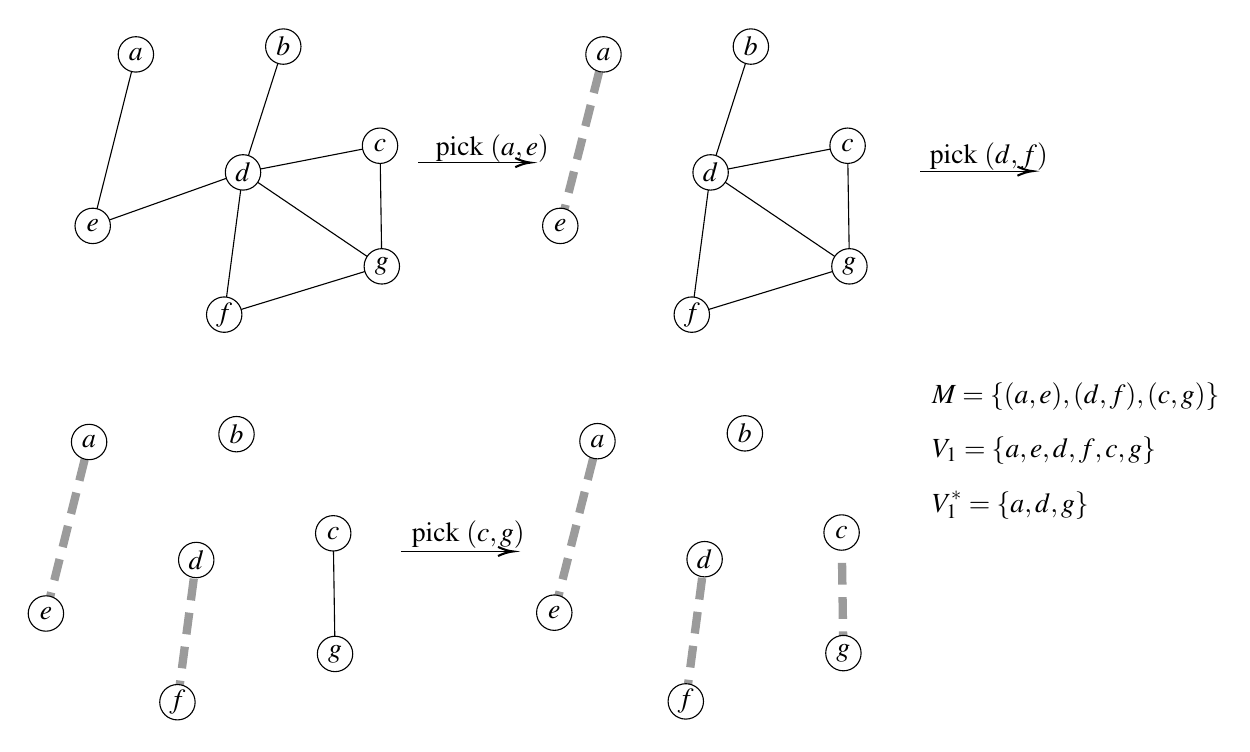
\begin{tikzpicture}[x=0.5pt,y=0.5pt,yscale=-1,xscale=1]
%uncomment if require: \path (0,509); %set diagram left start at 0, and has height of 509

%Straight Lines [id:da8273794433294758] 
\draw [color={rgb, 255:red, 155; green, 155; blue, 155 }  ,draw opacity=1 ][line width=3]  [dash pattern={on 7.88pt off 4.5pt}]  (386.16,427.29) -- (417.37,303.35) ;
%Straight Lines [id:da19729544641931185] 
\draw [color={rgb, 255:red, 155; green, 155; blue, 155 }  ,draw opacity=1 ][line width=3]  [dash pattern={on 7.88pt off 4.5pt}]  (481.2,491.42) -- (494.8,388.63) ;
%Straight Lines [id:da1947854045852928] 
\draw [color={rgb, 255:red, 155; green, 155; blue, 155 }  ,draw opacity=1 ][line width=3]  [dash pattern={on 7.88pt off 4.5pt}]  (595.1,456.53) -- (593.8,369.36) ;
%Straight Lines [id:da9648063665102072] 
\draw [color={rgb, 255:red, 155; green, 155; blue, 155 }  ,draw opacity=1 ][line width=3]  [dash pattern={on 7.88pt off 4.5pt}]  (113.81,492.01) -- (127.4,389.23) ;
%Straight Lines [id:da9576652196411746] 
\draw [color={rgb, 255:red, 155; green, 155; blue, 155 }  ,draw opacity=1 ][line width=3]  [dash pattern={on 7.88pt off 4.5pt}]  (18.77,427.89) -- (49.98,303.95) ;
%Straight Lines [id:da8239887263259694] 
\draw    (598.14,89.84) -- (499.14,109.11) ;
%Straight Lines [id:da8680955835635338] 
\draw    (485.54,211.9) -- (499.14,109.11) ;
%Straight Lines [id:da6116440428437093] 
\draw    (599.45,177.01) -- (485.54,211.9) ;
%Straight Lines [id:da2663821751343478] 
\draw    (599.45,177.01) -- (499.14,109.11) ;
%Straight Lines [id:da19351840074215054] 
\draw    (161.22,109.11) -- (260.22,89.84) ;
%Straight Lines [id:da43489413938826404] 
\draw    (161.22,109.11) -- (261.52,177.01) ;
%Straight Lines [id:da3853598268579197] 
\draw    (190.31,18.18) -- (161.22,109.11) ;
%Straight Lines [id:da21713072329995364] 
\draw    (261.52,177.01) -- (260.22,89.84) ;
%Straight Lines [id:da5478715757735835] 
\draw    (147.62,211.9) -- (261.52,177.01) ;
%Straight Lines [id:da42879006771456607] 
\draw    (52.58,147.77) -- (161.22,109.11) ;
%Straight Lines [id:da6771300098351073] 
\draw    (52.58,147.77) -- (83.79,23.83) ;
%Straight Lines [id:da4776548669152245] 
\draw    (147.62,211.9) -- (161.22,109.11) ;
%Shape: Ellipse [id:dp651117123053256] 
\draw  [fill={rgb, 255:red, 255; green, 255; blue, 255 }  ,fill opacity=1 ] (71,23.83) .. controls (71,16.77) and (76.73,11.04) .. (83.79,11.04) .. controls (90.86,11.04) and (96.58,16.77) .. (96.58,23.83) .. controls (96.58,30.9) and (90.86,36.62) .. (83.79,36.62) .. controls (76.73,36.62) and (71,30.9) .. (71,23.83) -- cycle ;
%Shape: Ellipse [id:dp7399561756845123] 
\draw  [fill={rgb, 255:red, 255; green, 255; blue, 255 }  ,fill opacity=1 ] (177.52,18.18) .. controls (177.52,11.11) and (183.25,5.39) .. (190.31,5.39) .. controls (197.38,5.39) and (203.1,11.11) .. (203.1,18.18) .. controls (203.1,25.24) and (197.38,30.97) .. (190.31,30.97) .. controls (183.25,30.97) and (177.52,25.24) .. (177.52,18.18) -- cycle ;
%Shape: Ellipse [id:dp8268258265249401] 
\draw  [fill={rgb, 255:red, 255; green, 255; blue, 255 }  ,fill opacity=1 ] (247.43,89.84) .. controls (247.43,82.78) and (253.15,77.05) .. (260.22,77.05) .. controls (267.28,77.05) and (273.01,82.78) .. (273.01,89.84) .. controls (273.01,96.9) and (267.28,102.63) .. (260.22,102.63) .. controls (253.15,102.63) and (247.43,96.9) .. (247.43,89.84) -- cycle ;
%Shape: Ellipse [id:dp5421818862330341] 
\draw  [fill={rgb, 255:red, 255; green, 255; blue, 255 }  ,fill opacity=1 ] (148.43,109.11) .. controls (148.43,102.05) and (154.15,96.32) .. (161.22,96.32) .. controls (168.28,96.32) and (174.01,102.05) .. (174.01,109.11) .. controls (174.01,116.18) and (168.28,121.9) .. (161.22,121.9) .. controls (154.15,121.9) and (148.43,116.18) .. (148.43,109.11) -- cycle ;
%Shape: Ellipse [id:dp45600813719389455] 
\draw  [fill={rgb, 255:red, 255; green, 255; blue, 255 }  ,fill opacity=1 ] (39.79,147.77) .. controls (39.79,140.71) and (45.52,134.98) .. (52.58,134.98) .. controls (59.64,134.98) and (65.37,140.71) .. (65.37,147.77) .. controls (65.37,154.84) and (59.64,160.56) .. (52.58,160.56) .. controls (45.52,160.56) and (39.79,154.84) .. (39.79,147.77) -- cycle ;
%Shape: Ellipse [id:dp031187496945339066] 
\draw  [fill={rgb, 255:red, 255; green, 255; blue, 255 }  ,fill opacity=1 ] (134.83,211.9) .. controls (134.83,204.83) and (140.56,199.11) .. (147.62,199.11) .. controls (154.69,199.11) and (160.41,204.83) .. (160.41,211.9) .. controls (160.41,218.96) and (154.69,224.69) .. (147.62,224.69) .. controls (140.56,224.69) and (134.83,218.96) .. (134.83,211.9) -- cycle ;
%Shape: Ellipse [id:dp7474313144054212] 
\draw  [fill={rgb, 255:red, 255; green, 255; blue, 255 }  ,fill opacity=1 ] (248.73,177.01) .. controls (248.73,169.94) and (254.46,164.22) .. (261.52,164.22) .. controls (268.59,164.22) and (274.31,169.94) .. (274.31,177.01) .. controls (274.31,184.07) and (268.59,189.8) .. (261.52,189.8) .. controls (254.46,189.8) and (248.73,184.07) .. (248.73,177.01) -- cycle ;
%Straight Lines [id:da10915523795701287] 
\draw    (528.24,18.18) -- (499.14,109.11) ;
%Straight Lines [id:da6013659372024278] 
\draw    (599.45,177.01) -- (598.14,89.84) ;
%Straight Lines [id:da2476997276246733] 
\draw [color={rgb, 255:red, 155; green, 155; blue, 155 }  ,draw opacity=1 ][line width=3]  [dash pattern={on 7.88pt off 4.5pt}]  (390.5,147.77) -- (421.72,23.83) ;
%Shape: Ellipse [id:dp27040633021074256] 
\draw  [fill={rgb, 255:red, 255; green, 255; blue, 255 }  ,fill opacity=1 ] (408.93,23.83) .. controls (408.93,16.77) and (414.65,11.04) .. (421.72,11.04) .. controls (428.78,11.04) and (434.51,16.77) .. (434.51,23.83) .. controls (434.51,30.9) and (428.78,36.62) .. (421.72,36.62) .. controls (414.65,36.62) and (408.93,30.9) .. (408.93,23.83) -- cycle ;
%Shape: Ellipse [id:dp9153562797015269] 
\draw  [fill={rgb, 255:red, 255; green, 255; blue, 255 }  ,fill opacity=1 ] (515.45,18.18) .. controls (515.45,11.11) and (521.17,5.39) .. (528.24,5.39) .. controls (535.3,5.39) and (541.03,11.11) .. (541.03,18.18) .. controls (541.03,25.24) and (535.3,30.97) .. (528.24,30.97) .. controls (521.17,30.97) and (515.45,25.24) .. (515.45,18.18) -- cycle ;
%Shape: Ellipse [id:dp47379487417600374] 
\draw  [fill={rgb, 255:red, 255; green, 255; blue, 255 }  ,fill opacity=1 ] (585.35,89.84) .. controls (585.35,82.78) and (591.07,77.05) .. (598.14,77.05) .. controls (605.2,77.05) and (610.93,82.78) .. (610.93,89.84) .. controls (610.93,96.9) and (605.2,102.63) .. (598.14,102.63) .. controls (591.07,102.63) and (585.35,96.9) .. (585.35,89.84) -- cycle ;
%Shape: Ellipse [id:dp7207828118279439] 
\draw  [fill={rgb, 255:red, 255; green, 255; blue, 255 }  ,fill opacity=1 ] (486.35,109.11) .. controls (486.35,102.05) and (492.08,96.32) .. (499.14,96.32) .. controls (506.2,96.32) and (511.93,102.05) .. (511.93,109.11) .. controls (511.93,116.18) and (506.2,121.9) .. (499.14,121.9) .. controls (492.08,121.9) and (486.35,116.18) .. (486.35,109.11) -- cycle ;
%Shape: Ellipse [id:dp7155442322771159] 
\draw  [fill={rgb, 255:red, 255; green, 255; blue, 255 }  ,fill opacity=1 ] (377.71,147.77) .. controls (377.71,140.71) and (383.44,134.98) .. (390.5,134.98) .. controls (397.57,134.98) and (403.29,140.71) .. (403.29,147.77) .. controls (403.29,154.84) and (397.57,160.56) .. (390.5,160.56) .. controls (383.44,160.56) and (377.71,154.84) .. (377.71,147.77) -- cycle ;
%Shape: Ellipse [id:dp4818001756043101] 
\draw  [fill={rgb, 255:red, 255; green, 255; blue, 255 }  ,fill opacity=1 ] (472.75,211.9) .. controls (472.75,204.83) and (478.48,199.11) .. (485.54,199.11) .. controls (492.61,199.11) and (498.33,204.83) .. (498.33,211.9) .. controls (498.33,218.96) and (492.61,224.69) .. (485.54,224.69) .. controls (478.48,224.69) and (472.75,218.96) .. (472.75,211.9) -- cycle ;
%Shape: Ellipse [id:dp9764479331484588] 
\draw  [fill={rgb, 255:red, 255; green, 255; blue, 255 }  ,fill opacity=1 ] (586.66,177.01) .. controls (586.66,169.94) and (592.38,164.22) .. (599.45,164.22) .. controls (606.51,164.22) and (612.24,169.94) .. (612.24,177.01) .. controls (612.24,184.07) and (606.51,189.8) .. (599.45,189.8) .. controls (592.38,189.8) and (586.66,184.07) .. (586.66,177.01) -- cycle ;
%Straight Lines [id:da7079754945425016] 
\draw    (227.71,457.12) -- (226.4,369.95) ;
%Shape: Ellipse [id:dp8120027238634924] 
\draw  [fill={rgb, 255:red, 255; green, 255; blue, 255 }  ,fill opacity=1 ] (37.19,303.95) .. controls (37.19,296.88) and (42.92,291.16) .. (49.98,291.16) .. controls (57.04,291.16) and (62.77,296.88) .. (62.77,303.95) .. controls (62.77,311.01) and (57.04,316.74) .. (49.98,316.74) .. controls (42.92,316.74) and (37.19,311.01) .. (37.19,303.95) -- cycle ;
%Shape: Ellipse [id:dp23465413123771173] 
\draw  [fill={rgb, 255:red, 255; green, 255; blue, 255 }  ,fill opacity=1 ] (143.71,298.29) .. controls (143.71,291.23) and (149.44,285.5) .. (156.5,285.5) .. controls (163.56,285.5) and (169.29,291.23) .. (169.29,298.29) .. controls (169.29,305.35) and (163.56,311.08) .. (156.5,311.08) .. controls (149.44,311.08) and (143.71,305.35) .. (143.71,298.29) -- cycle ;
%Shape: Ellipse [id:dp6697870946666823] 
\draw  [fill={rgb, 255:red, 255; green, 255; blue, 255 }  ,fill opacity=1 ] (213.61,369.95) .. controls (213.61,362.89) and (219.34,357.16) .. (226.4,357.16) .. controls (233.47,357.16) and (239.19,362.89) .. (239.19,369.95) .. controls (239.19,377.02) and (233.47,382.74) .. (226.4,382.74) .. controls (219.34,382.74) and (213.61,377.02) .. (213.61,369.95) -- cycle ;
%Shape: Ellipse [id:dp6678250120125151] 
\draw  [fill={rgb, 255:red, 255; green, 255; blue, 255 }  ,fill opacity=1 ] (114.61,389.23) .. controls (114.61,382.16) and (120.34,376.44) .. (127.4,376.44) .. controls (134.47,376.44) and (140.19,382.16) .. (140.19,389.23) .. controls (140.19,396.29) and (134.47,402.02) .. (127.4,402.02) .. controls (120.34,402.02) and (114.61,396.29) .. (114.61,389.23) -- cycle ;
%Shape: Ellipse [id:dp44880213332154095] 
\draw  [fill={rgb, 255:red, 255; green, 255; blue, 255 }  ,fill opacity=1 ] (5.98,427.89) .. controls (5.98,420.83) and (11.7,415.1) .. (18.77,415.1) .. controls (25.83,415.1) and (31.56,420.83) .. (31.56,427.89) .. controls (31.56,434.95) and (25.83,440.68) .. (18.77,440.68) .. controls (11.7,440.68) and (5.98,434.95) .. (5.98,427.89) -- cycle ;
%Shape: Ellipse [id:dp5261031453835676] 
\draw  [fill={rgb, 255:red, 255; green, 255; blue, 255 }  ,fill opacity=1 ] (101.02,492.01) .. controls (101.02,484.95) and (106.75,479.22) .. (113.81,479.22) .. controls (120.87,479.22) and (126.6,484.95) .. (126.6,492.01) .. controls (126.6,499.07) and (120.87,504.8) .. (113.81,504.8) .. controls (106.75,504.8) and (101.02,499.07) .. (101.02,492.01) -- cycle ;
%Shape: Ellipse [id:dp96264308088132] 
\draw  [fill={rgb, 255:red, 255; green, 255; blue, 255 }  ,fill opacity=1 ] (214.92,457.12) .. controls (214.92,450.06) and (220.65,444.33) .. (227.71,444.33) .. controls (234.77,444.33) and (240.5,450.06) .. (240.5,457.12) .. controls (240.5,464.18) and (234.77,469.91) .. (227.71,469.91) .. controls (220.65,469.91) and (214.92,464.18) .. (214.92,457.12) -- cycle ;
%Shape: Ellipse [id:dp08371522903251905] 
\draw  [fill={rgb, 255:red, 255; green, 255; blue, 255 }  ,fill opacity=1 ] (404.58,303.35) .. controls (404.58,296.29) and (410.31,290.56) .. (417.37,290.56) .. controls (424.44,290.56) and (430.16,296.29) .. (430.16,303.35) .. controls (430.16,310.42) and (424.44,316.14) .. (417.37,316.14) .. controls (410.31,316.14) and (404.58,310.42) .. (404.58,303.35) -- cycle ;
%Shape: Ellipse [id:dp16754302978302682] 
\draw  [fill={rgb, 255:red, 255; green, 255; blue, 255 }  ,fill opacity=1 ] (511.11,297.7) .. controls (511.11,290.63) and (516.83,284.91) .. (523.9,284.91) .. controls (530.96,284.91) and (536.69,290.63) .. (536.69,297.7) .. controls (536.69,304.76) and (530.96,310.48) .. (523.9,310.48) .. controls (516.83,310.48) and (511.11,304.76) .. (511.11,297.7) -- cycle ;
%Shape: Ellipse [id:dp8803652600651565] 
\draw  [fill={rgb, 255:red, 255; green, 255; blue, 255 }  ,fill opacity=1 ] (581.01,369.36) .. controls (581.01,362.3) and (586.73,356.57) .. (593.8,356.57) .. controls (600.86,356.57) and (606.59,362.3) .. (606.59,369.36) .. controls (606.59,376.42) and (600.86,382.15) .. (593.8,382.15) .. controls (586.73,382.15) and (581.01,376.42) .. (581.01,369.36) -- cycle ;
%Shape: Ellipse [id:dp08434869719365379] 
\draw  [fill={rgb, 255:red, 255; green, 255; blue, 255 }  ,fill opacity=1 ] (482.01,388.63) .. controls (482.01,381.57) and (487.74,375.84) .. (494.8,375.84) .. controls (501.86,375.84) and (507.59,381.57) .. (507.59,388.63) .. controls (507.59,395.7) and (501.86,401.42) .. (494.8,401.42) .. controls (487.74,401.42) and (482.01,395.7) .. (482.01,388.63) -- cycle ;
%Shape: Ellipse [id:dp8697258636657205] 
\draw  [fill={rgb, 255:red, 255; green, 255; blue, 255 }  ,fill opacity=1 ] (373.37,427.29) .. controls (373.37,420.23) and (379.1,414.5) .. (386.16,414.5) .. controls (393.23,414.5) and (398.95,420.23) .. (398.95,427.29) .. controls (398.95,434.36) and (393.23,440.08) .. (386.16,440.08) .. controls (379.1,440.08) and (373.37,434.36) .. (373.37,427.29) -- cycle ;
%Shape: Ellipse [id:dp3796179832525568] 
\draw  [fill={rgb, 255:red, 255; green, 255; blue, 255 }  ,fill opacity=1 ] (468.41,491.42) .. controls (468.41,484.35) and (474.14,478.63) .. (481.2,478.63) .. controls (488.27,478.63) and (493.99,484.35) .. (493.99,491.42) .. controls (493.99,498.48) and (488.27,504.21) .. (481.2,504.21) .. controls (474.14,504.21) and (468.41,498.48) .. (468.41,491.42) -- cycle ;
%Shape: Ellipse [id:dp22651898621493904] 
\draw  [fill={rgb, 255:red, 255; green, 255; blue, 255 }  ,fill opacity=1 ] (582.32,456.53) .. controls (582.32,449.46) and (588.04,443.74) .. (595.1,443.74) .. controls (602.17,443.74) and (607.89,449.46) .. (607.89,456.53) .. controls (607.89,463.59) and (602.17,469.32) .. (595.1,469.32) .. controls (588.04,469.32) and (582.32,463.59) .. (582.32,456.53) -- cycle ;
%Straight Lines [id:da8565598108716722] 
\draw    (287.8,102.04) -- (366.89,102.04) ;
\draw [shift={(368.89,102.04)}, rotate = 180] [color={rgb, 255:red, 0; green, 0; blue, 0 }  ][line width=0.75]    (10.93,-3.29) .. controls (6.95,-1.4) and (3.31,-0.3) .. (0,0) .. controls (3.31,0.3) and (6.95,1.4) .. (10.93,3.29)   ;
%Straight Lines [id:da8466299980928367] 
\draw    (650.72,108.21) -- (729.82,108.21) ;
\draw [shift={(731.82,108.21)}, rotate = 180] [color={rgb, 255:red, 0; green, 0; blue, 0 }  ][line width=0.75]    (10.93,-3.29) .. controls (6.95,-1.4) and (3.31,-0.3) .. (0,0) .. controls (3.31,0.3) and (6.95,1.4) .. (10.93,3.29)   ;
%Straight Lines [id:da6943383967058451] 
\draw    (275.35,383.05) -- (354.44,383.05) ;
\draw [shift={(356.44,383.05)}, rotate = 180] [color={rgb, 255:red, 0; green, 0; blue, 0 }  ][line width=0.75]    (10.93,-3.29) .. controls (6.95,-1.4) and (3.31,-0.3) .. (0,0) .. controls (3.31,0.3) and (6.95,1.4) .. (10.93,3.29)   ;

% Text Node
\draw (657.36,298.36) node [anchor=north west][inner sep=0.75pt]   [align=left] {$\displaystyle V_{1} =\{a,e,d,f,c,g\}$};
% Text Node
\draw (657.36,337.59) node [anchor=north west][inner sep=0.75pt]   [align=left] {$\displaystyle V^{*}_{1} =\{a,d,g\}$};
% Text Node
\draw (83.79,23.83) node   [align=left] {$\displaystyle a$};
% Text Node
\draw (190.31,18.18) node   [align=left] {$\displaystyle b$};
% Text Node
\draw (260.22,89.84) node   [align=left] {$\displaystyle c$};
% Text Node
\draw (161.22,109.11) node   [align=left] {$\displaystyle d$};
% Text Node
\draw (52.58,147.77) node   [align=left] {$\displaystyle e$};
% Text Node
\draw (147.62,211.9) node   [align=left] {$\displaystyle f$};
% Text Node
\draw (261.52,177.01) node   [align=left] {$\displaystyle g$};
% Text Node
\draw (421.72,23.83) node   [align=left] {$\displaystyle a$};
% Text Node
\draw (528.24,18.18) node   [align=left] {$\displaystyle b$};
% Text Node
\draw (598.14,89.84) node   [align=left] {$\displaystyle c$};
% Text Node
\draw (499.14,109.11) node   [align=left] {$\displaystyle d$};
% Text Node
\draw (390.5,147.77) node   [align=left] {$\displaystyle e$};
% Text Node
\draw (485.54,211.9) node   [align=left] {$\displaystyle f$};
% Text Node
\draw (599.45,177.01) node   [align=left] {$\displaystyle g$};
% Text Node
\draw (49.98,303.95) node   [align=left] {$\displaystyle a$};
% Text Node
\draw (156.5,298.29) node   [align=left] {$\displaystyle b$};
% Text Node
\draw (226.4,369.95) node   [align=left] {$\displaystyle c$};
% Text Node
\draw (127.4,389.23) node   [align=left] {$\displaystyle d$};
% Text Node
\draw (18.77,427.89) node   [align=left] {$\displaystyle e$};
% Text Node
\draw (113.81,492.01) node   [align=left] {$\displaystyle f$};
% Text Node
\draw (227.71,457.12) node   [align=left] {$\displaystyle g$};
% Text Node
\draw (417.37,303.35) node   [align=left] {$\displaystyle a$};
% Text Node
\draw (523.9,297.7) node   [align=left] {$\displaystyle b$};
% Text Node
\draw (593.8,369.36) node   [align=left] {$\displaystyle c$};
% Text Node
\draw (494.8,388.63) node   [align=left] {$\displaystyle d$};
% Text Node
\draw (386.16,427.29) node   [align=left] {$\displaystyle e$};
% Text Node
\draw (481.2,491.42) node   [align=left] {$\displaystyle f$};
% Text Node
\draw (595.1,456.53) node   [align=left] {$\displaystyle g$};
% Text Node
\draw (298.71,79.84) node [anchor=north west][inner sep=0.75pt]   [align=left] {pick $\displaystyle ( a,e)$};
% Text Node
\draw (655.68,86.01) node [anchor=north west][inner sep=0.75pt]   [align=left] {pick $\displaystyle ( d,f)$};
% Text Node
\draw (281.28,358.84) node [anchor=north west][inner sep=0.75pt]   [align=left] {pick $\displaystyle ( c,g)$};
% Text Node
\draw (657.36,259.13) node [anchor=north west][inner sep=0.75pt]   [align=left] {$\displaystyle M=\{( a,e) ,( d,f) ,( c,g)\}$};


\end{tikzpicture}

}
\caption{Running the edge-based greedy algorithm on this instance:
the picked edges and the graph $(V, E_1)$ in each iteration is illustrated. 
The greedy algorithm returns $V_1$, while the optimal solution is $V_1^*$.}
\label{fig:greedy2}
\end{figure}

Is this greedy algorithm an approximation algorithm? Again yes, and it commits
a (much) better approximation ratio of 2!
\begin{fact}
Let $V_1$ be the vertex cover returned by above (edge-based) greedy algorithm.
Let $V_1^*$ be the optimal vertex cover.
We have $|V_1| \le 2 |V_1^*|$.
\end{fact}
\emph{Proof.} First, notice that $|V_1| = 2|M|$, as both end-vertices
of an edge in $M$ will be added to $V_1$. Second, edges in $M$ don't
share vertices. (In other words, $M$ is a \emph{matching}; a matching
is defined as a set of edges that don't share vertices.)
Therefore, in order to cover these edges in $M$, at least
one end-vertex of each edge in $M$ needs to be included.
Hence, any vertex cover will contain at least $|M|$ vertices.
This of course applies to the optimal vertex cover, i.e., $|V_1^*| \ge |M|$.
Combined, we have $|V_1| = 2|M| \le 2|V_1^*|$.  \qed

\end{document}
